% OrganPrompt -- arXiv preprint
% Build:  cd paper && pdflatex main && bibtex main && pdflatex main && pdflatex main
% (or:    python ../scripts/build_paper.py)
\documentclass[11pt]{article}

\usepackage[letterpaper,margin=1in]{geometry}
\usepackage[T1]{fontenc}
\usepackage[utf8]{inputenc}
\usepackage{lmodern}
\usepackage{microtype}
\usepackage{amsmath,amssymb}
\usepackage{graphicx}
\usepackage{booktabs}
\usepackage{tabularx}
\usepackage{makecell}
\usepackage{enumitem}
\usepackage{float}      % [H] for floats that must not drift out of their section
\usepackage[section]{placeins}  % keep floats inside the section that introduces them
\usepackage{multirow}
\usepackage{siunitx}
\usepackage[font=small,labelfont=bf]{caption}
\usepackage{subcaption}
\usepackage{xcolor}
\usepackage{authblk}
\usepackage[numbers,sort&compress]{natbib}
\usepackage[colorlinks=true,linkcolor=blue!55!black,citecolor=blue!55!black,
            urlcolor=blue!55!black]{hyperref}
\usepackage{xurl}   % allow long URLs to break anywhere rather than overflow

\graphicspath{{../figures/}{../figures/paper/}{../diagnostics/}}

% Numbers in tables: right-aligned on the decimal point.
\sisetup{detect-weight=true,detect-inline-weight=math}
\newcommand{\org}[1]{\texttt{#1}}          % organ class names
\newcommand{\code}[1]{\texttt{#1}}

\title{\bfseries OrganPrompt: Weakly-Supervised Text-Prompted\\
       Organ Localization in CT, and Its Use as a\\
       Bone-Metastasis Proximity Index}

% TODO(authors): add the second author. Name, affiliation and order need to come
% from you. Uncomment the marked lines and fill in.
\author[1]{Arnav Sangle}
% \author[2]{<Given name> Du}
\affil[1]{\small [affiliation to be added]}
% \affil[2]{\small <affiliation>}
\affil[ ]{\small Correspondence: \href{mailto:arnavsangle08@gmail.com}{arnavsangle08@gmail.com}}

% No date. Empty \date{} suppresses it entirely; do NOT use \today, which would
% stamp the build date and change on every recompile.
\date{}

\begin{document}
\maketitle

\begin{abstract}
Dense per-voxel annotation is the binding constraint on CT segmentation.
Vision--language models trained on image--text pairs offer a route around it,
but their contrastive objective aligns pooled image and caption embeddings, so
individual patch tokens are never required to be spatially discriminative:
reading per-patch similarity off such a model recovers 0.003 mIoU. We make that
spatial property an explicit training objective, aligning each ViT patch token
with the organ's text embedding against a downsampled mask, so per-patch cosine
similarity becomes directly readable as a segmentation map at inference, with no
gradients, no classifier, and no second-stage mask refiner. On 11 organ classes
from TotalSegmentator this reaches 0.653 mIoU and 0.757 Dice using no per-pixel
labels at inference; a calibration correction contributes 0.059 of that with no
retraining. A prompt ablation shows the text is load-bearing rather than a class
index, since corrupting positional language collapses exactly the classes that
depend on laterality and leaves uniquely-positioned organs unaffected. The same
ablation shows elaboration is not where the value lies: a bare class name
recovers 96.9\% of a full multi-sentence anatomical description, and a one-line
generic caption matches it outright. An accidental two-word prompt error
revealed that failures are directional rather than degradative, producing a
confident, clean segmentation of the wrong organ, which is the more dangerous
failure mode because nothing in the output signals it. Carrying the frozen model
onto an unseen dataset and protocol, we compute a bone-metastasis proximity
index over Spine-Mets-CT-SEG: across 180 lesions in 46 patients the correct
organ ranks 1.78 on average against a chance rank of 2.91 ($p < 0.0001$,
patient-clustered permutation test), beating chance at every level from T1 to
T11 and concentrating its failures in two of eleven classes. We
report two pre-registered calibration variants that were run and not adopted,
each with a diagnosed mechanism, along with a ground-truth error in our own
evaluation table found and corrected from anatomical literature, and a
calibration leak found and repaired. Both corrections changed headline numbers.

\end{abstract}

\section{Introduction}
\label{sec:intro}

Dense per-voxel annotation is the binding constraint on CT segmentation. A
fully supervised model such as TotalSegmentator already segments more than a
hundred anatomical structures at a level of agreement comparable to an expert
reader \cite{wasserthal2023totalsegmentator}, so accuracy is not the open
problem; that performance instead rests entirely on expert voxel-level labels
for every structure of interest. Because it is the labels rather than the
architecture that determine which structures such a system can recognize,
extending it to a new structure, a new protocol, or a new clinical question
means commissioning new annotation.

That commissioning is expensive because voxel-level delineation of CT is not
unskilled work. It requires a reader trained in cross-sectional anatomy who can
identify organ boundaries on axial slices where soft-tissue contrast is often
poor and where adjacent structures share intensity, and such expertise is
correspondingly scarce and costly to secure. The burden also scales
multiplicatively rather than additively, since every structure must be traced on
every slice of every volume, and a single CT volume comprises hundreds of
slices. As a result, densely labeled CT datasets are few in number, and each
one is fixed in the label set that a particular funding decision chose to
support \cite{ji2022amos, luo2022word, rister2020ctorg}, which means a structure
outside that set is simply unavailable to anyone working from it. A second
consequence follows from the same difficulty: where expert judgment is genuinely
ambiguous, as it is at low-contrast boundaries, even careful annotators
disagree, and therefore the ground truth against which these models are trained
and scored itself carries reader variability \cite{nikolov2021nsd}. The
limitation that matters here is consequently not model capacity but the
annotation itself, which raises the question of whether the supervision might
instead be drawn from a source that already exists rather than one that has to
be created.

Text is the natural candidate for such a source, because descriptions of
anatomy are already abundant in clinical reports and in the biomedical
literature, and vision--language pretraining offers a means of learning from
them. Models in the CLIP family learn visual concepts from natural-language
supervision alone \cite{radford2021clip, zhai2023siglip}, and biomedical
adaptations such as PMC-CLIP \cite{lin2023pmcclip} and BiomedCLIP
\cite{zhang2025biomedclip} bring that capability into the medical domain at
scale. If a text prompt could select a region as well as it selects a label,
segmentation would need no pixels at all.

The obstacle is that these models are trained for global alignment. The
contrastive objective relates a pooled image embedding to a pooled caption
embedding, and nothing in it requires an individual patch token to be spatially
discriminative. The conventional way to recover a spatial map from a trained
network is the CAM family \cite{zhou2016cam, selvaraju2017gradcam}, which
extracts one post hoc from a classifier; that route is closed here, however,
because a contrastively pretrained model makes no per-organ decision for a CAM
to explain. What remains available is to backpropagate the image--text
similarity to the input pixels, and that gradient saliency recovers almost no
localization: applied to the pretrained model, it reaches 0.003 mIoU.

This work makes the spatial property an explicit training objective instead.
That objective aligns each of the 196 ViT patch tokens with the organ's text
embedding against the downsampled ground-truth mask, so that per-patch cosine
similarity becomes directly readable as a segmentation map at inference. Because
the map is read straight off the forward pass, the method requires no gradient
computation, no classifier, and no second-stage mask refiner. The contributions
are as follows.

\textbf{A patch-level alignment objective that makes text-prompted localization
work.} Aligning each patch token directly with the organ's text embedding
reaches 0.653 mIoU on 11 organ classes from TotalSegmentator while requiring no
per-pixel labels at inference, and the patch loss contributes more of that
localization than any other component of the method
(\S\ref{sec:results:phase1}).

\textbf{A prompt ablation that establishes what the text is actually doing, and
what it is not.} Corrupting the positional content of the prompts collapses
precisely the classes that depend on laterality while leaving
uniquely-positioned organs untouched, which establishes that the prompt is
load-bearing rather than acting as a class index
(\S\ref{sec:results:ablation}).

\textbf{A safety-relevant failure mode.} An accidental two-word error in one of
eleven prompts produced not a degraded output but a confident, clean
segmentation of the wrong organ, which means that failures of this method are
directional rather than degradative and are therefore unsignaled by the output
itself (\S\ref{sec:results:ablation}).

\textbf{A downstream clinical application of the frozen model.} Carried
unmodified onto Spine-Mets-CT-SEG \cite{pieper2024spinemets}, a dataset and
acquisition protocol never seen in training, the same weights rank the organ
nearest a vertebral metastasis well above chance across 180 lesions in 46
patients, at $p < 0.0001$ under a patient-clustered permutation test
(\S\ref{sec:results:lesion}).

\textbf{Negative results with diagnosed mechanisms.} Neither of two
pre-registered calibration variants was adopted, in each case for an identified
reason rather than for an unexplained regression
(\S\ref{sec:results:negatives}) -- a diagnosis that extends to the residual
localization failure itself, which is not diffuse but concentrates in two of
eleven classes (\S\ref{sec:discussion}).

We also report a ground-truth error that we found in our own evaluation table
and corrected from anatomical literature, together with a calibration leak that
we found and repaired. Because both of these changed headline numbers,
reporting them is part of what the paper claims rather than an aside to it.

\section{Related work}
\label{sec:related}

\subsection{Vision--language pretraining and its biomedical adaptations}

Conventional recognition models are trained against a fixed, closed set of
labels chosen in advance, so every additional category requires fresh labeled
examples and usually a new output layer. Vision--language pretraining replaces
that arrangement with a joint embedding space for images and free text, learned
by contrastively aligning large corpora of image--caption pairs, so that a
category is specified at inference by writing it in natural language rather than
by having been enumerated at training time. The supervision is not free, since
captions are themselves human-written text paired with images, but it is
open-vocabulary, and that property is what makes the paradigm attractive for a
problem in which the structures of interest are not fixed in advance.

CLIP established that predicting which caption belongs to which image, over 400
million web-collected pairs, yields representations strong enough for zero-shot
transfer across more than 30 vision benchmarks \cite{radford2021clip}. SigLIP
later replaced the softmax-normalized contrastive objective with a pairwise
sigmoid loss that needs no global view of the similarity matrix, which decouples
the loss from batch size and improves results at both small and very large
batches \cite{zhai2023siglip}.

Much of the subsequent progress has been attributed to data rather than
architecture. MetaCLIP argues explicitly that CLIP's principal ingredient is its
curation procedure, and recovers CLIP-level performance by balancing a raw pool
against metadata derived from CLIP's own concept list \cite{xu2024metaclip}.
DataComp makes the same point by construction, fixing the training code and
treating the dataset as the object of study across a 12.8-billion-pair candidate
pool \cite{gadre2023datacomp}. Both results motivate the biomedical variants,
where the binding constraint is domain-matched data.

Two such adaptations are directly relevant. PMC-CLIP assembles PMC-OA, 1.6M
image--caption pairs from PubMed Central's Open Access subset, most aligned at
subfigure and subcaption granularity \cite{lin2023pmcclip}. BiomedCLIP scales
this further with PMC-15M, 15 million figure--caption pairs drawn from 4.4
million articles, and adapts the text side to the domain: a PubMedBERT encoder
with a 30k domain-specific vocabulary in place of a general-domain tokenizer,
and a context length raised to 256 tokens to accommodate the length of PMC
captions \cite{zhang2025biomedclip}. That longer context is what makes
multi-sentence anatomical prompts expressible at all, and this work builds on
BiomedCLIP for that reason.

What none of these models supplies, however, is spatial grounding, and the
reason is worth setting out as a diagnosis rather than a complaint, because
these models are behaving exactly as their objective specifies. That objective
constrains only the pooled image representation against the pooled caption
representation: the pooled vector is what is projected into the shared embedding
space and scored, and individual patch tokens enter the loss only indirectly,
through whatever the pooling operation draws from them. No gradient therefore
ever asks a particular patch token to align with the text on its own, which
means a model can minimize the objective perfectly while its patch tokens hold
representations that are useful for assembling the pooled summary yet not
individually meaningful when compared against a text embedding. Two further
properties of the architecture compound this. The projection head is fit to the
distribution of pooled representations, so pushing patch tokens through that
same head asks it to do something it was never trained for; and self-attention
in the deeper blocks mixes information globally, so a late-layer patch token
reflects image-wide context rather than the evidence at its own location, which
is precisely the locality a similarity map would need.

That the pooling stage is implicated is not a new observation. MaskCLIP
recovers a substantial amount of dense signal by reading CLIP's value projection
instead of the attention-pooled output \cite{zhou2022maskclip}, later work in
the same line pushes that recovery further \cite{yang2025clipdense}, and
methods that re-pose the objective at pixel level \cite{rao2022denseclip} or
attach a decoder trained for the purpose \cite{lueddecke2022clipseg} restore
dense behavior by other means. Read naively, then, per-patch similarity from a
CLS-trained model has no reason to carry a localization signal, and the
untrained pipeline recovers almost none: gradient saliency on the pretrained
model reaches 0.003 mIoU before any fine-tuning (\S\ref{sec:results}). The
question this work takes up is what supplies the gradient pressure the
pretraining objective never had reason to apply.

\subsection{Dense and local alignment from vision--language models}

Those repairs are worth separating out, because global alignment has been
identified as the obstacle before, and the closest work attacks it in three
distinguishable ways.

The first extracts dense correspondence from an already-trained model without
changing its weights. MaskCLIP shows that CLIP's value projection retains
substantially more spatial information than the pooled embedding suggests, and
recovers usable dense labels by reading it directly \cite{zhou2022maskclip}.
Subsequent work pushes this further for weakly supervised semantic segmentation
\cite{yang2025clipdense}, and a related line examines why CLIP's raw attention
localizes poorly and how its explainability can be repaired
\cite{li2024clipexplain}. Self-supervised vision transformers exhibit a similar
property, with DINO producing segmentation-like attention maps without any
textual supervision \cite{caron2021dino}. OrganPrompt takes the same view of
where the signal lives but trains the property in rather than recovering it,
because the downstream index requires organ maps that vanish where the organ is
absent, which is a calibration property rather than a localization one.

The second, instead of reading the signal out of frozen weights, adapts the
model to dense prediction with a task head. DenseCLIP converts image-text
matching into pixel-text matching and fine-tunes with a dense decoder
\cite{rao2022denseclip}, and CLIPSeg attaches a lightweight transformer decoder
that emits a segmentation from a text or image prompt
\cite{lueddecke2022clipseg}. Both produce better boundaries than OrganPrompt,
but both also place a trained decoder between the prompt and the mask, which is
precisely the attribution problem described below.

The third builds the local property in during pretraining rather than adding it
afterwards, and GLoRIA is the closest medical antecedent: it learns global and
local representations jointly by matching image sub-regions to individual words
in radiology reports \cite{huang2021gloria}. The objective here is the same in
spirit, but it differs in supervision and in target, because GLoRIA attends over
report words to build localized representations for label-efficient recognition,
whereas we supervise each of the 196 patch tokens directly against a downsampled
organ mask, so that the resulting per-patch similarity is itself the
segmentation rather than an intermediate representation.

\subsection{Text-driven medical image segmentation}

Within text-driven medical segmentation itself, the closest methodological
relative is MedCLIP-SAMv2, which shares both the BiomedCLIP backbone and the
premise that a text prompt can drive segmentation
\cite{koleilat2025medclipsamv2}, extending an earlier version of the same
framework \cite{koleilat2024medclipsam}. It differs in where the mask comes from:
saliency derived from the vision--language model is used to prompt SAM
\cite{kirillov2023sam}, which produces the final boundary, in a lineage that
includes MedSAM's adaptation of SAM to medical images \cite{ma2024medsam}.

Delegating mask formation to a second model, as that lineage does, is the
stronger engineering choice and generally yields better boundaries, but it also
changes what the pipeline can be asked. When a refiner sits between the prompt
and the output, a failure cannot be attributed cleanly to the text, because the
refiner may repair a bad localization or corrupt a good one. Reading patch
similarity directly, as here, gives up boundary quality and gains attribution in
exchange: the caption ablation in \S\ref{sec:results:ablation} is only
interpretable because nothing stands between the prompt and the mask. We regard
that trade as the substantive difference between the two approaches, not the
scores in Table~\ref{tab:weaksup}, which are computed on different datasets and
organ sets.

\subsection{Weak supervision, stratified by annotation cost}

That lineage and OrganPrompt are both weakly supervised in the broad sense,
which is exactly the problem: ``weakly supervised'' covers a wide range of
supervision strength, and comparing across that range without saying so is
misleading.
Point-supervised methods receive one clicked pixel inside each structure;
scribble-supervised methods receive a stroke through it. Recent work in this
tier reports substantial gains
over prior point- and scribble-supervised baselines on BTCV and CHAOS
\cite{jiang2024probabilistic}. Multi-organ abdominal CT benchmarks such as AMOS
\cite{ji2022amos} and WORD \cite{luo2022word} are the usual evaluation targets in
this tier, which is one reason no row of Table~\ref{tab:weaksup} shares a dataset
with the evaluation here.

What point and scribble annotation have in common is that both answer ``where''
for each training image. Image-level text supervision does not answer it at all,
which is the entire problem being solved here, so these methods are context
rather than baselines. The strictly comparable tier is instead image-level
supervision, where weakly supervised CAM-based lesion segmentation in PET-CT
reports a median Dice of 0.47 against 0.72 for a fully supervised U-Net
\cite{ronneberger2015unet} on the same task \cite{fruh2021petct}, the fully
supervised tier in which transformer architectures such as TransUNet
\cite{chen2021transunet} are now a common alternative. That ratio, roughly two
thirds of supervised performance recovered from image-level labels alone, is the
expectation this work should be read against.

\subsection{Class activation maps and post-hoc localization}

The image-level tier has an established localization technique of its own, and
it starts from a classifier rather than from a vision--language model: the CAM
family. CAM recovers localization from a classifier's final-layer activations
\cite{zhou2016cam}, and Grad-CAM generalizes this to arbitrary architectures by
weighting activations with backpropagated gradients \cite{selvaraju2017gradcam},
with later refinements such as Grad-CAM++ improving multi-instance localization
\cite{chattopadhay2018gradcampp}. What every member of the family has in common
is that it explains where a trained classifier looked.

That shared framing is what makes the family a poor fit here, for a reason worth
stating plainly rather than asserting. A CAM explains a decision the network
already makes, and a contrastively pretrained vision--language model makes no
per-organ decision to explain, because it produces an embedding whose alignment
with a text embedding is a similarity rather than a class logit. Applying
gradient-based localization to it consequently recovers almost nothing, which is
what the 0.003 starting point in Table~\ref{tab:progression} measures. Because
there is no decision to explain, this work trains the spatial property directly
instead of attempting to extract it post hoc, and the name reflects that: the
prompt does the localizing, and no activation map is involved.

\subsection{Positioning}

Those observations locate this work. It sits in the image-level tier and differs
from its nearest neighbors in three respects, the first of which the preceding
subsection has already anticipated. It trains patch-level text--image alignment
as an explicit objective instead of extracting localization post hoc from a
classifier. It reads the resulting similarity map directly, with no second-stage
refiner, which preserves the ability to attribute failures to the prompt. And it
carries the same frozen model into a downstream
clinical question, the bone-metastasis proximity index of
\S\ref{sec:results:index}, on a dataset and acquisition protocol the model never
saw during training.

One point of provenance completes that picture. The underlying idea was
validated on the OrganAMNIST subset of MedMNIST v2 \cite{yang2023medmnist}
before the move to full-resolution CT; the results here are on the latter only.

\section{Methods}
\label{sec:methods}

\subsection{Backbone and fine-tuning}
\label{sec:methods:backbone}

We start from BioMedCLIP \cite{zhang2025biomedclip}, which pairs a ViT-B/16
visual encoder \cite{dosovitskiy2021vit} with a PubMedBERT text encoder
\cite{gu2021pubmedbert}, 195M parameters in total:

\begin{center}
\small\path{hf-hub:microsoft/BiomedCLIP-PubMedBERT_256-vit_base_patch16_224}
\end{center}

We freeze the entire model and then selectively unfreeze by name: ViT blocks
8--11, PubMedBERT encoder layers 8--11, \code{visual.head}, \code{text.proj},
\code{logit\_scale} and \code{logit\_bias}, roughly 57M of 195M parameters. We
keep \code{visual.head} trainable because it is the projection our patch-level
loss (\S\ref{sec:methods:patchloss}) computes through. Freezing it would
decouple the patch objective from the representation it is meant to shape.

We optimize with AdamW at a peak learning rate of $10^{-4}$ and weight decay
0.01, using 200 steps of linear warmup followed by cosine annealing, with batch
size 32. Each version in Table~\ref{tab:progression} is a 20-epoch run resumed
from the previous checkpoint rather than a fresh initialization.

\begin{figure}[t]
\centering
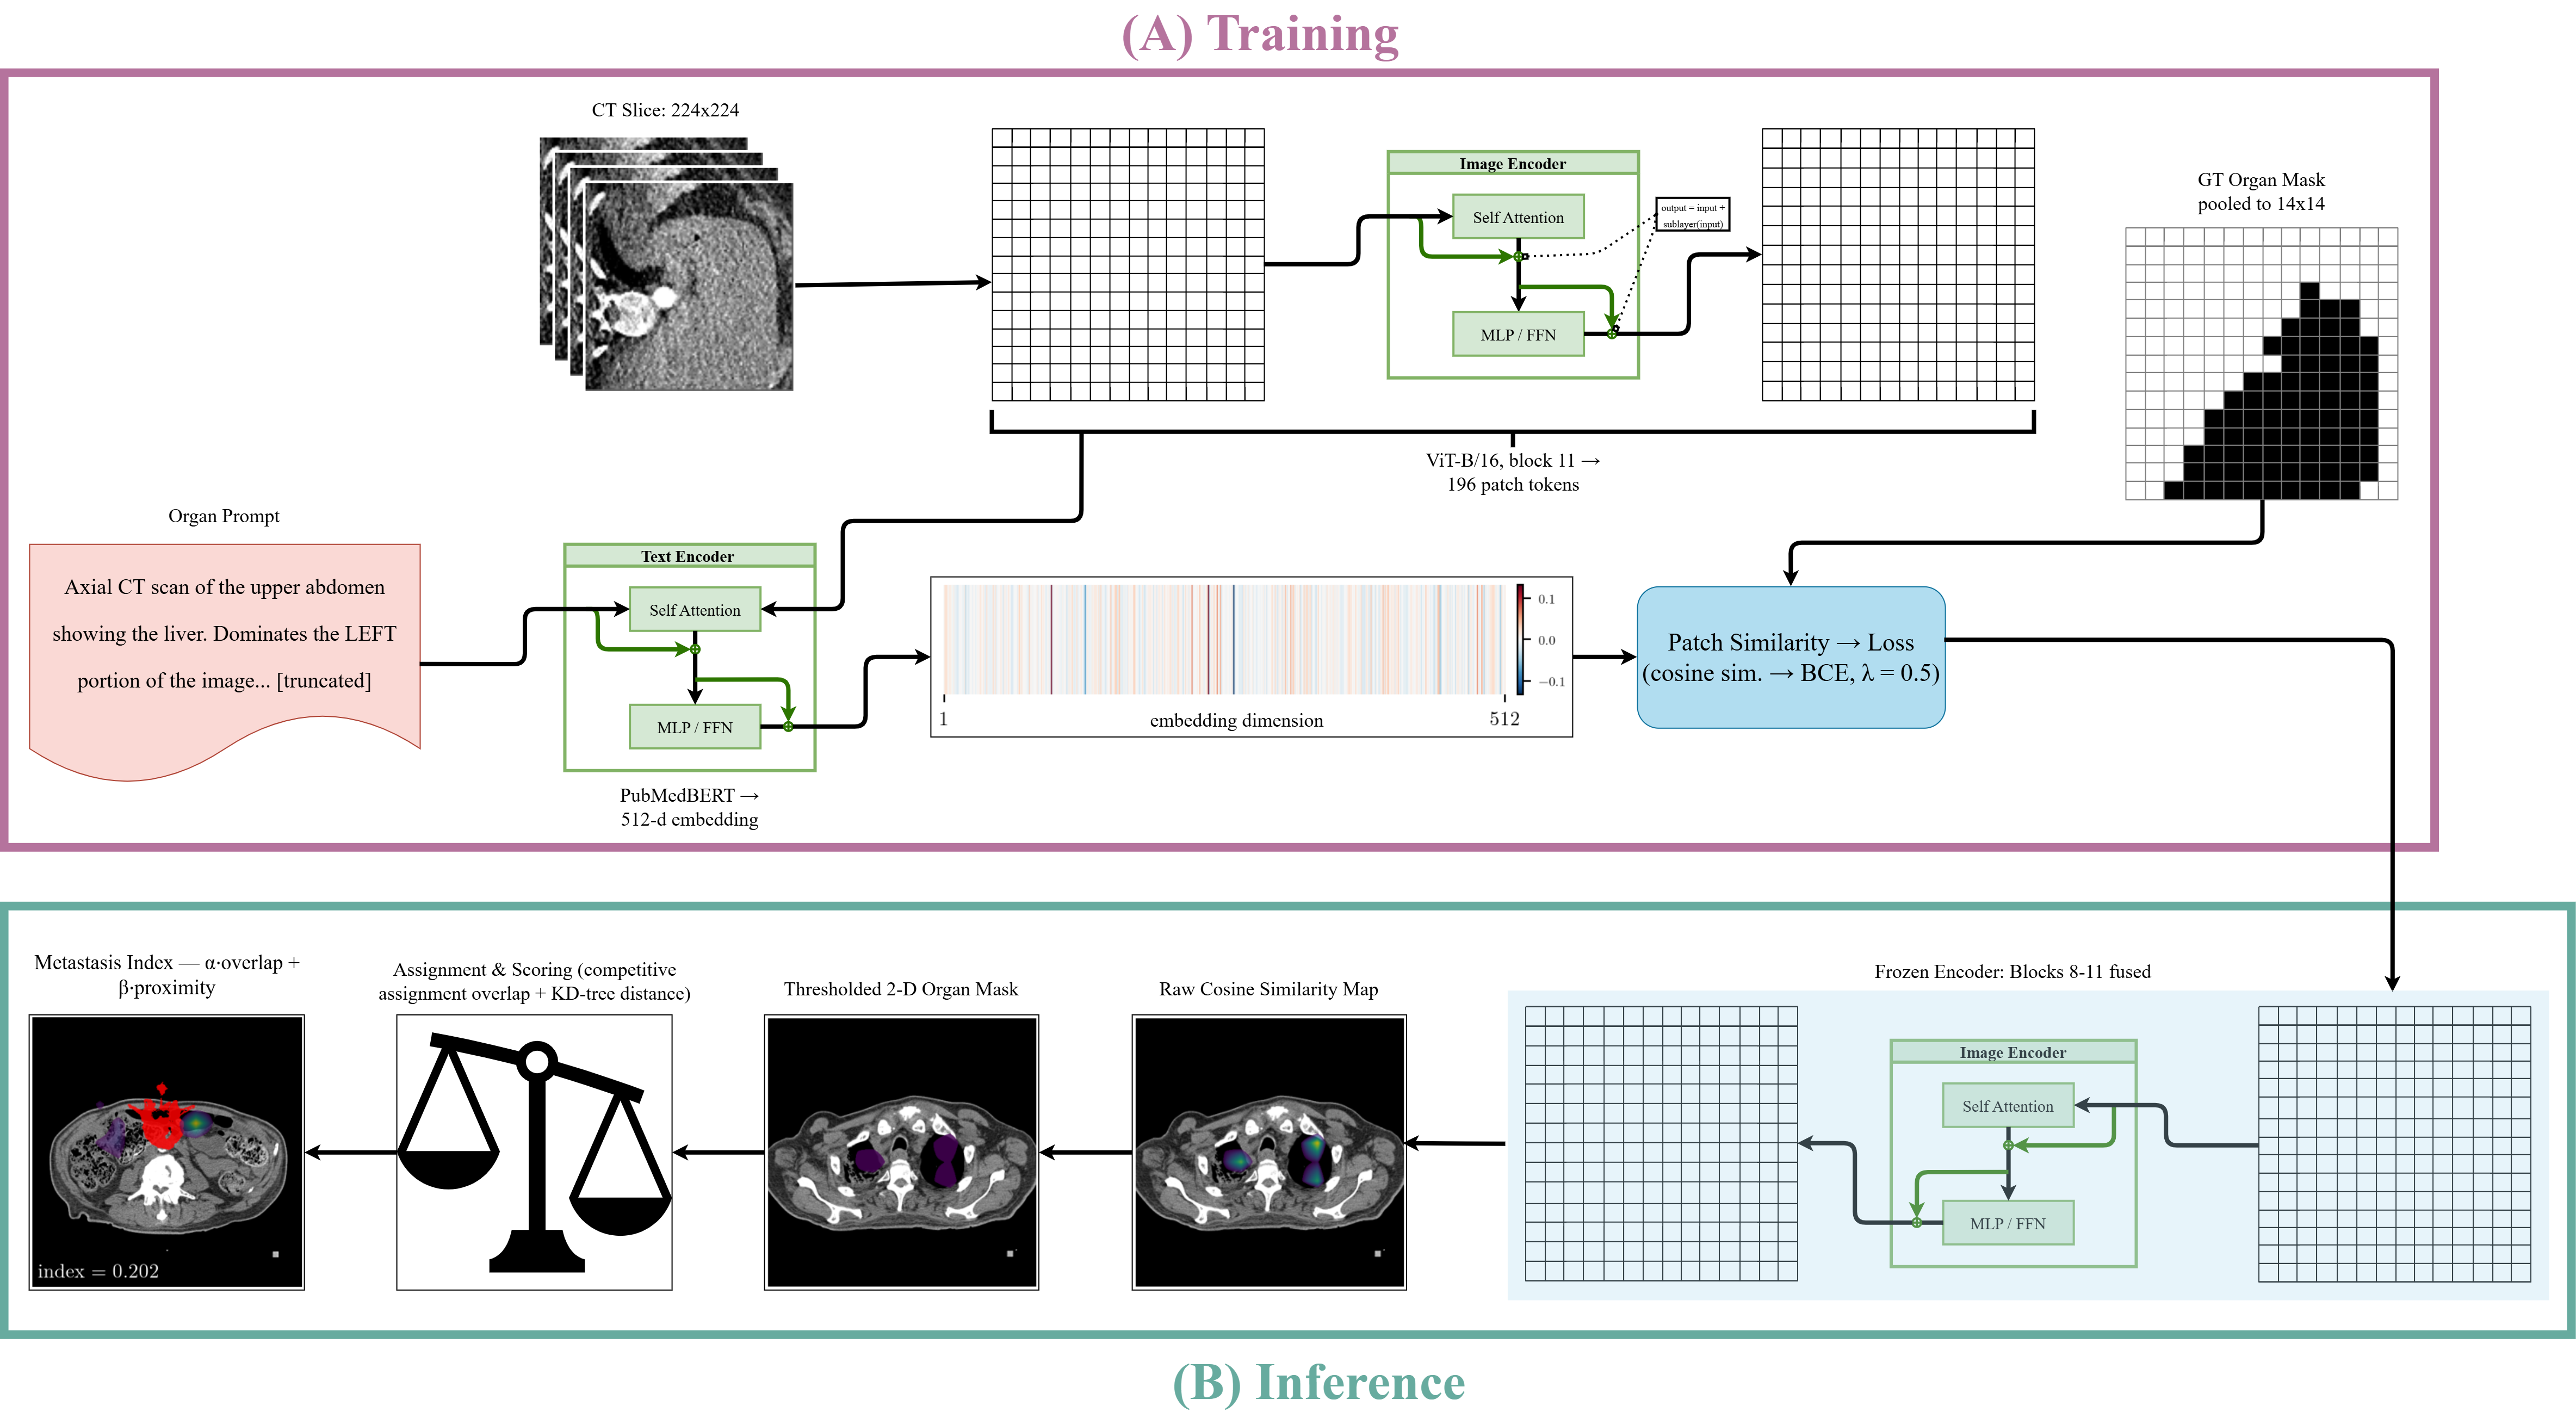
\includegraphics[width=\textwidth]{fig0_pipeline.png}
\caption{Method overview. \textbf{(A)} Training. A forward hook on ViT block 11
captures 196 patch tokens, which we project through \code{visual.head} and
$L_2$-normalize; the ground-truth organ mask is area-pooled to the same
$14\times14$ grid, and a per-patch binary cross-entropy against the organ's text
embedding supervises every patch rather than only the pooled CLS token.
\textbf{(B)} Inference. No gradients, no classifier and no mask refiner are
involved: blocks 8--11 are averaged, per-patch cosine similarity is read
directly, upsampled and thresholded per class, then stacked across axial slices
into a 3D volume. Competitive assignment awards each voxel to at most one organ,
so an organ that loses its own peak is reported absent, and the surviving masks
are scored against each lesion by overlap and KD-tree distance to give the
proximity index. Colour marks the image path (blue), text path (orange),
similarity and mask path (green), and loss or index (vermilion).}
\label{fig:pipeline}
\end{figure}

\subsection{Patch-level contrastive objective}
\label{sec:methods:patchloss}

This is the central methodological component and, empirically, the single
largest contributor to performance (Table~\ref{tab:progression});
Figure~\ref{fig:pipeline}A shows it schematically. CLS-level
contrastive training aligns a whole image with a whole caption. Nothing in that
objective requires any individual patch token to be discriminative, so patch-text
similarity from a CLS-trained model is close to unusable as a segmentation map.
The patch loss supplies the missing constraint.

We register a forward hook on ViT block 11 to capture the block's output as a
side effect of the ordinary forward pass, and drop the CLS token to leave 196
patch tokens of dimension 768. We project these through \code{visual.head} to
512 dimensions and $L_2$-normalize them. We downsample the ground-truth mask to
the $14\times14$ patch grid by area interpolation, using average pooling rather
than nearest-neighbour so that a thin structure is not aliased into or out of
existence, and binarize at 0.5 to give one label per patch. Writing $e_p$ for
the normalized embedding of patch $p$, $t$ for the $L_2$-normalized organ text
embedding, $s$ for the learned logit scale and $y_p \in \{0,1\}$ for the patch
label, our loss is

\begin{equation}
\mathcal{L}_{\text{patch}}
  = \frac{1}{196}\sum_{p=1}^{196}
    \mathrm{BCE}\!\left(s \cdot \langle e_p, t\rangle,\; y_p\right),
\qquad
\mathcal{L} = \mathcal{L}_{\text{SigLIP}} + \lambda\,\mathcal{L}_{\text{patch}},
\end{equation}

with $\lambda = 0.5$. Patches inside the organ are pulled toward the organ's
text embedding and patches outside are pushed away, which makes per-patch
similarity directly readable as a spatial map.

\paragraph{Resolution constraint.}
Patch supervision is fixed at $14\times14$ by the ViT-B/16 geometry at
$224\times224$ input. Boundary precision is therefore inherently coarse, and the
HD95 of 18.8 pixels in Table~\ref{tab:overall} substantially reflects the
upsampled patch grid rather than gross mislocalization. This is an architectural property of the backbone, not an unturned knob.

\subsection{Inference: multi-layer patch-similarity fusion}
\label{sec:methods:inference}

Figure~\ref{fig:pipeline}B summarizes the inference path, which differs from
training in three ways: four blocks are fused instead of one, no mask is
involved, and no gradient is computed.
At inference we need no gradients. We hook ViT blocks 8, 9, 10 and 11 to capture
each block's token output, average the four, drop the CLS token, and project the
resulting 196 patch tokens through \code{visual.head} with $L_2$-normalization,
exactly as in training. The map for organ $c$ is the raw cosine similarity
$\langle e_p, t_c\rangle$ per patch, reshaped to $14\times14$ and bilinearly
upsampled to $224\times224$.

We average four blocks rather than using the final block alone because this
combines the semantic response of blocks 10--11 with the finer texture and edge
response of blocks 8--9, which improves boundary localization.

We also implement an optional hard-negative variant that subtracts the strongest
competing response, $\text{CAM}_p = \langle e_p, t_c\rangle - \max_{n} \langle
e_p, t_n\rangle$ over a set of negative prompts. This is the mechanism we test
and do not adopt in \S\ref{sec:results:negatives}. Our default configuration
does not use it.

\subsection{Calibration: two removed defaults}
\label{sec:methods:calibration}

We found two conventional choices to be actively harmful and removed both. The
resulting $+0.059$ mIoU (Table~\ref{tab:progression}, v4~$\to$~v4-tuned)
required no retraining.

\textbf{We removed per-image min--max normalization.} Rescaling each slice's map
to $[0,1]$ forces every slice to span the full dynamic range whether or not the
organ is present, which destroys exactly the confidence information that
distinguishes ``this organ is here'' from ``this organ is absent from this
slice.'' The maps are therefore raw cosine similarities, bounded in $[-1,1]$ and
routinely negative across an entire slice (Figure~\ref{fig:rawsim}). Organs win
relatively, not absolutely. Every visualization in this paper thresholds at a percentile of the
slice's own distribution for this reason.

\begin{figure}[t]
\centering
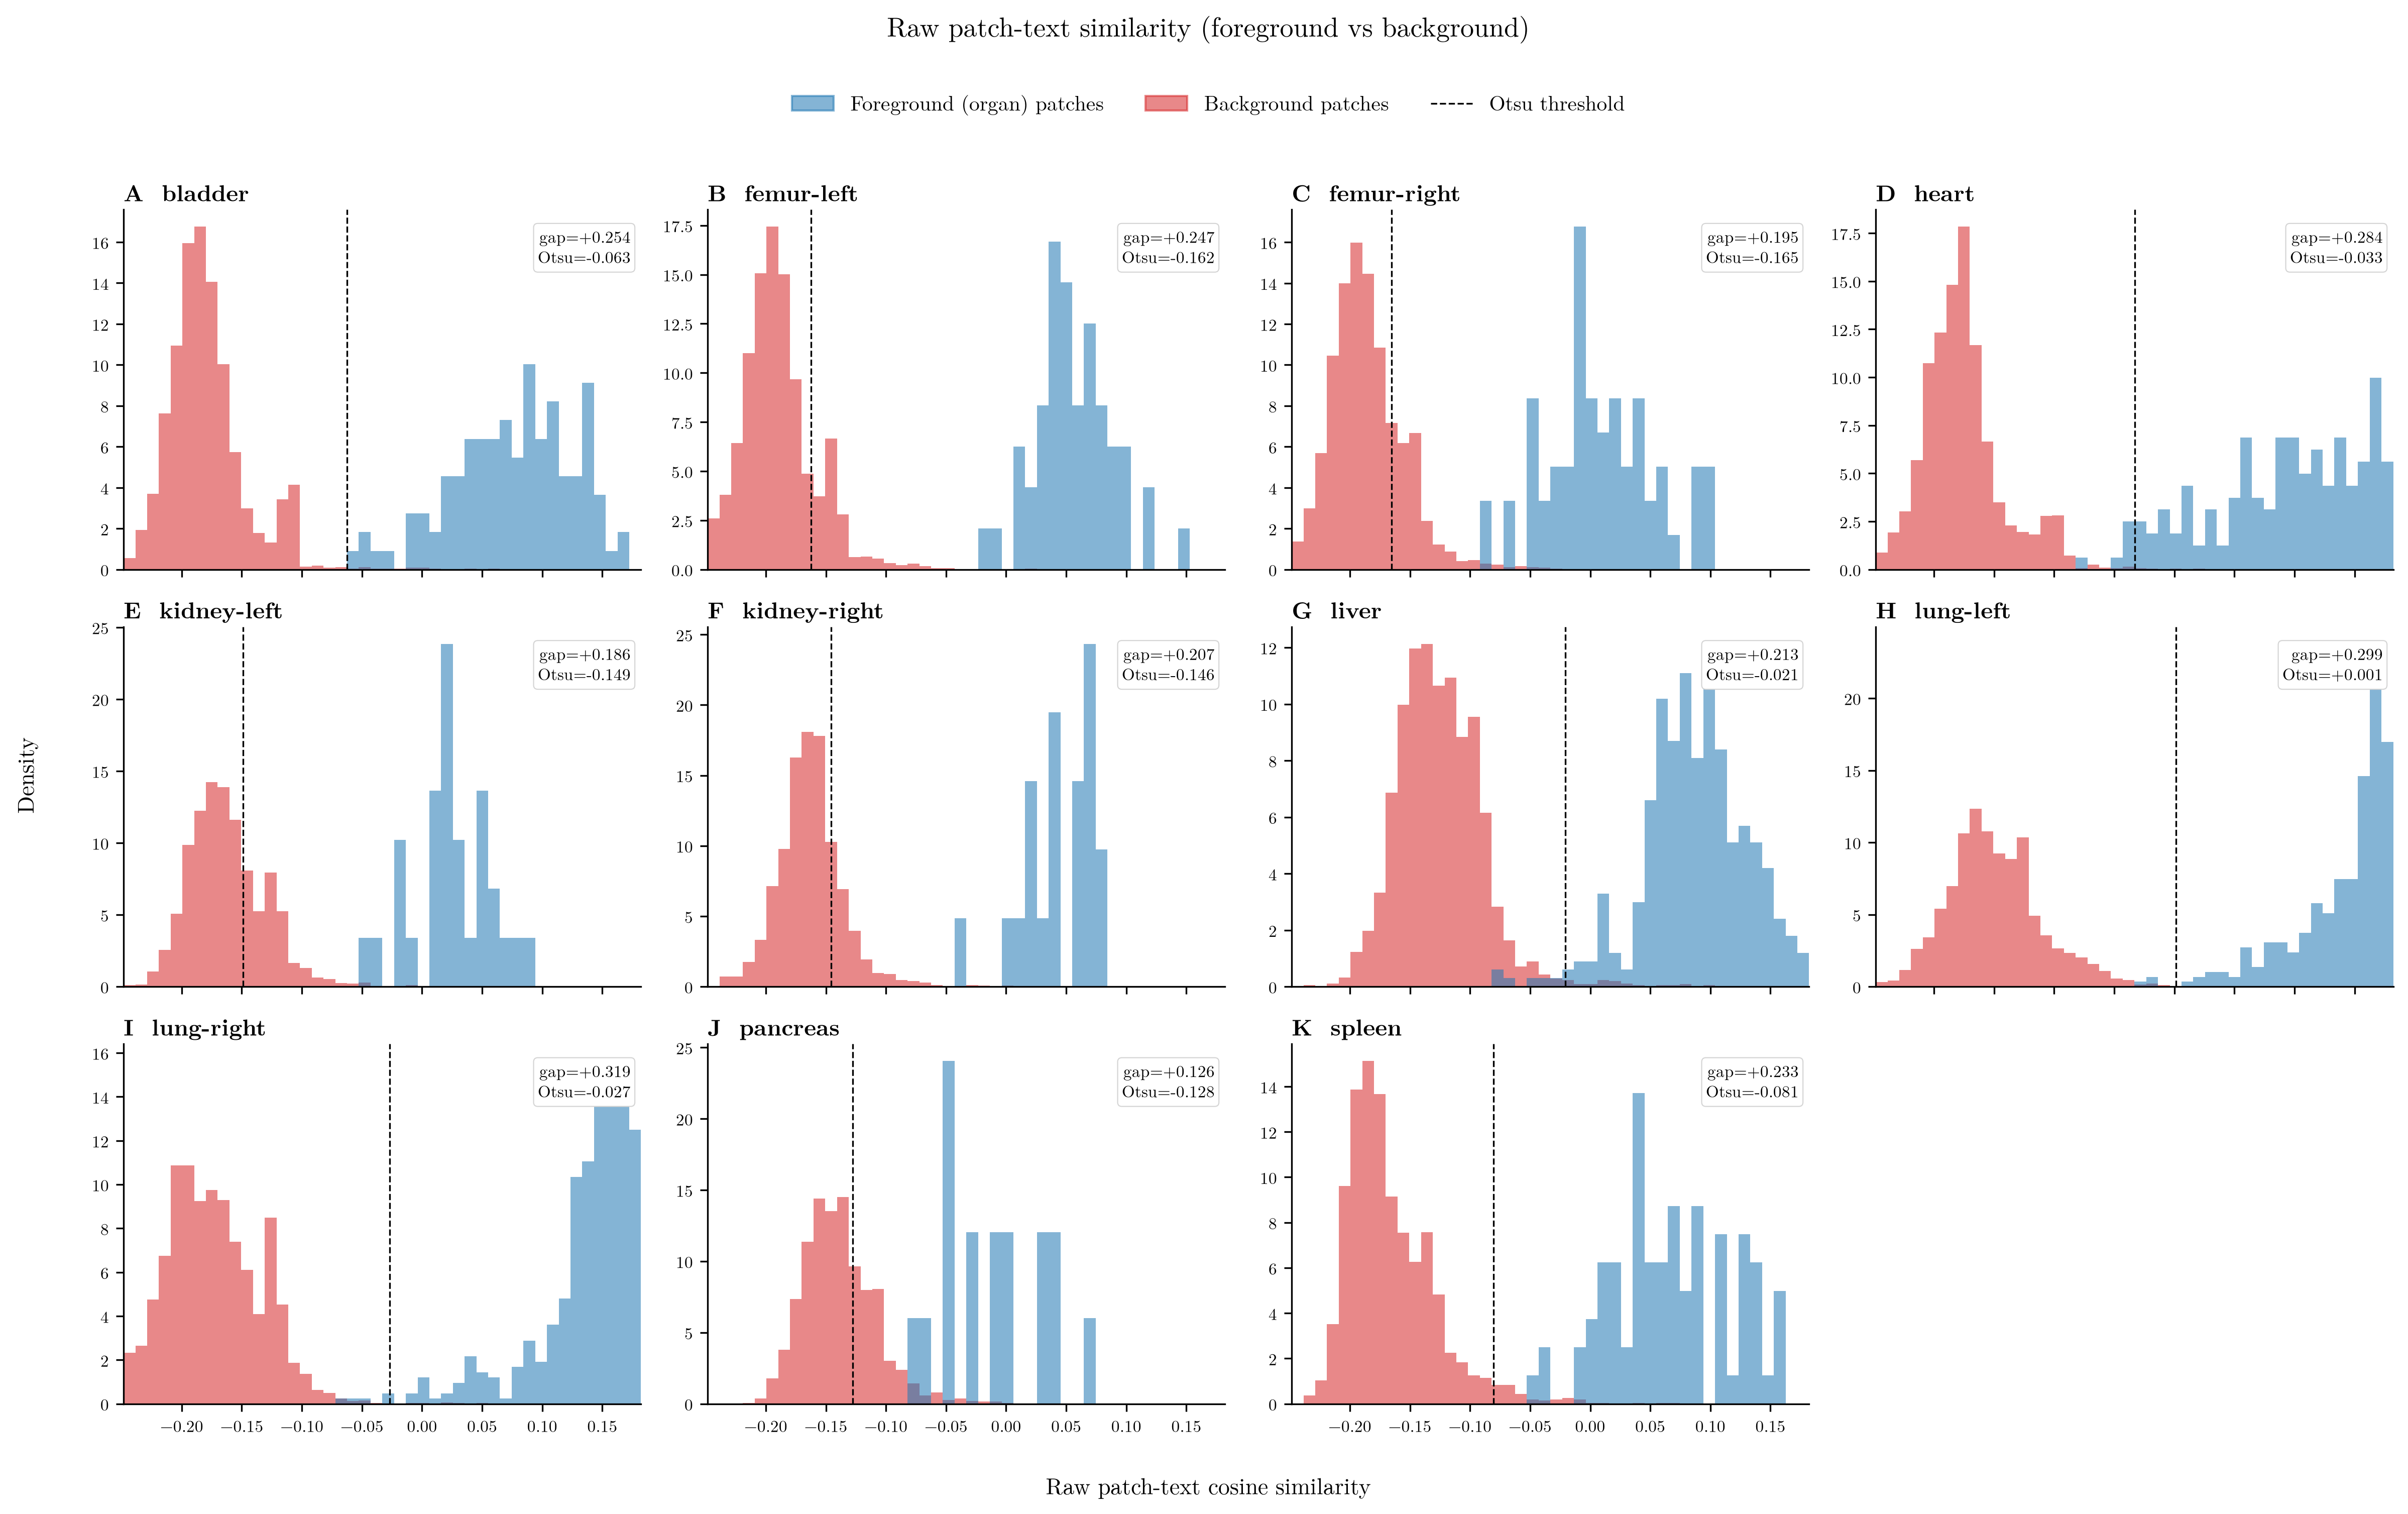
\includegraphics[width=0.72\textwidth]{raw_similarities.png}
\caption{Raw patch-text similarity distributions per organ class, before any
normalization. The distributions are bounded in $[-1,1]$, sit largely below
zero, and differ in location and spread from class to class. Both facts drive
the calibration decisions in this section: because the maps are routinely
negative, an absolute-zero threshold is meaningless and every visualization in
this paper thresholds at a percentile of the slice's own distribution; and
because the classes are not on a common scale, cross-organ comparison requires
the per-organ calibration of \S\ref{sec:methods:assign} rather than a raw
argmax. Per-image min--max normalization would flatten exactly this structure.}
\label{fig:rawsim}
\end{figure}

\textbf{We removed class-conditional negative subtraction} from the default
path, having measured that it cuts more foreground signal than background.

In their place we calibrate per-class thresholds by sweeping IoU-optimal cutoffs
on generated masks. These thresholds are the only fitted quantity in the Phase~1 pipeline.

\subsection{Data and evaluation protocol}
\label{sec:methods:data}

We train and evaluate on TotalSegmentator v2.0.1
\cite{wasserthal2023totalsegdataset}: 1{,}228 thoracic and abdominal CT volumes
with per-voxel organ labels. We use eleven classes, forming the two lungs by
merging the released per-lobe labels (left $=$ upper $+$ lower; right $=$ upper
$+$ middle $+$ lower), so the lung classes are whole lungs.

We take the 80/10/10 split at the \emph{volume} level with a fixed seed, so no
slice from a training patient can appear at validation or test time. Within a
volume we index the top $K=5$ slices per organ, which concentrates supervision
on slices where the organ is substantially present.

We preprocess with an organ-dependent HU window ($[-1000, -200]$ for lungs,
$[-200, 1000]$ for femurs, $[-150, 250]$ otherwise), then rescale to $[0,1]$,
resize to $224\times224$ bilinearly, and replicate the single channel three
times to match the RGB-shaped input. We apply no rotation or flip augmentation.
Laterality is semantically meaningful for six of our eleven classes and is
carried explicitly by the prompts, so a horizontal flip would silently invert
the label.

We report 2D per-slice IoU and Dice on organ-present slices, plus HD95,
sensitivity, precision, relative volume error, and normalized surface Dice
\cite{nikolov2021nsd} at $\tau = 3$\,px. \textbf{This 2D, organ-present protocol is more forgiving than
3D volumetric scoring}, since no empty or partial-boundary slices dilute the
average, and every cross-paper comparison in \S\ref{sec:results:comparison}
inherits that caveat.

\paragraph{Checkpoint selection.}
Validation loss is the SigLIP CLS-level objective and does \emph{not} track
mIoU. A checkpoint can improve global image-text alignment while its patch maps
degrade. We therefore rank checkpoints by the full mask-metric suite computed on
generated masks, never by validation loss. We state this explicitly because the
default habit of taking the lowest-val-loss epoch selects the wrong checkpoint
here.

\subsection{Caption ablation design}
\label{sec:methods:captions}

To separate the prompt's contribution from the visual encoder's, we re-evaluated
the fine-tuned v4 model under five prompt formulations with the text embedding
as the only variable and no retraining (Table~\ref{tab:captions}): class name
only (L1), a generic clinical caption (L2), position language with the organ
name removed (L3), the full multi-sentence anatomical description used during
training (L4), and an adversarial variant (L5). We reproduce all five sets
verbatim in Appendix~\ref{app:prompts}.

We construct L5 as L4 with LEFT$\leftrightarrow$RIGHT and
top$\leftrightarrow$bottom exchanged. The design point is that this preserves
fluency, length, clause structure and every non-spatial anatomical claim while
inverting only the spatial content. A class that collapses under L5 must
therefore have been relying on the positional text, and a class that does not
must have been relying on something else. That contrast is what makes the
bilateral-versus-unilateral split in \S\ref{sec:results:ablation} interpretable
rather than merely suggestive.

One caveat belongs in the method rather than the results. Our L3 prompt for
\org{lung-right} was generated incorrectly, naming the left lung and the left
half of the image. We discovered this during analysis; we did not design it. We
report it in \S\ref{sec:results:ablation} as a natural experiment because the
error happens to be internally consistent, and therefore isolates what a
coherent but wrong prompt does, but it was not a controlled manipulation.

\subsection{Competitive cross-organ assignment}
\label{sec:methods:assign}

Applying our Phase~1 pipeline to whole volumes exposes a structural problem that
per-slice classification hides. Thresholding each organ's map independently
means \emph{every} organ always receives a mask. A bladder prompt run over a
chest CT still has a global maximum somewhere, so it claims the most
bladder-like thoracic tissue and reports itself present. Absence is not
expressible. We found that neither component size nor peak similarity separates
these phantoms from correct detections, since a correct spleen appeared at the
0th size percentile while a wrong bladder sat at the 65th, so no per-organ gate
can remove them.

Assignment by competition can. We award each voxel to at most one organ, the one
that responds most strongly there after calibration. An organ whose own best
voxel is claimed by a stronger organ is reported \textbf{absent} and receives no
mask, which is precisely the signal independent thresholding cannot produce. We
stream organs one at a time against a running best-value and best-label array,
so memory stays bounded regardless of organ count.

\paragraph{Calibration is required for the argmax to mean anything.}
Raw similarity is not comparable across prompts, since lungs peak near 0.18 and
femurs near 0.06, so an uncalibrated cross-organ argmax would hand nearly every
voxel to the lungs. Our default \emph{scale} mode divides each organ's map by
that organ's typical peak response, putting all organs on a common ``fraction of
the response this organ ever gives'' scale. We also implement a \emph{z-score}
mode computing $(\text{raw} - \mu_c)/\sigma_c$ per organ, which unlike the scale
mode corrects for baseline offset as well as scale. The z-score mode is the
variant we evaluate and do not adopt in \S\ref{sec:results:negatives}.

\paragraph{Bilateral pairs compete as one unit.}
Letting \org{kidney-left} and \org{kidney-right} bid against each other
reproduced the same bug one level down. The two prompts differ by a single
laterality word, the text encoder separates them poorly, both peak in nearly the
same place, and the stronger one declares the weaker absent. In an early
measurement 37\% of pairs split this way. A scan contains both sides of a pair
or neither, so we decide presence for the \emph{pair}: we record the winner as a
group identifier, and paired organs therefore never take territory from one
another. We then divide the group's won territory by position on the image
midline, using the convention our prompts state explicitly and consistently, in
which a patient-left organ ``appears on the RIGHT side of the image''.

\paragraph{Finalization.}
An organ's mask is the connected component of its group's won territory
containing that organ's own peak voxel, subject to a floor. Winning a voxel is
not sufficient: the calibrated value must also exceed 0.6, or every voxel in the
body would be assigned to something. When a member's peak falls in its pair's
half, which is routine given the laterality confusion above, we use the largest
component instead of returning nothing.

\subsection{Bone-metastasis proximity index}
\label{sec:methods:index}

The index reuses the Phase~1 model frozen and unmodified, on Spine-Mets-CT-SEG
\cite{pieper2024spinemets}: 55 patients of 3D DICOM CT with per-vertebra SEG
masks, of which 46 carry usable labels. We read lesion involvement per vertebral
level from the collection's clinical spreadsheet, \emph{not} from the SEG file,
and form the tumor mask as the union of vertebra masks for levels the
spreadsheet marks involved.

OrganPrompt is inherently 2D, so we preprocess each axial slice exactly as in
training, run it through the patch-similarity engine, and stack and resample the
resulting per-slice maps to the native in-plane resolution, giving a 3D organ
volume aligned to the CT grid. Competitive assignment
(\S\ref{sec:methods:assign}) then reduces that to mutually exclusive 3D organ
masks. Lesion voxels are vertebral bone by construction, so any organ predicted
\emph{at} the lesion is a model artifact. We carve those voxels out of every
organ mask before scoring, or a confused prediction would fake overlap with
itself.

For each (tumor, organ) pair we compute
\begin{equation}
\text{overlap} = \frac{|T \cap O|}{|T|},
\qquad
\text{proximity} = \frac{1}{1 + d_{\text{mm}}},
\qquad
\text{score} = \alpha\,\text{overlap} + \beta\,\text{proximity},
\end{equation}
with $\alpha = \beta = 0.5$, and take the patient's index as the maximum score
over organs, so the nearest or most-involved organ drives it. Here
$d_{\text{mm}}$ is the minimum physical distance between tumor and organ voxels,
which we obtain by building a KD-tree over organ voxel coordinates scaled by the
volume's mm spacing and querying it with the lesion's coordinates.

We deliberately do not use a Euclidean distance transform. The EDT allocates a
float64 array over the whole volume, on the order of 600\,MB per organ across 11
organs, purely to read a single minimum out of it, which is enough to exhaust
memory on a full-resolution scan. Both point sets are small, so the KD-tree
answers the same question exactly in a few MB. We do use the EDT, appropriately,
for the HD95 and NSD surface metrics of \S\ref{sec:methods:data}.

We fix $\alpha$, $\beta$ and the max-over-organs aggregation a priori and do not
fit them.

Before trusting the index at all, we checked our organ maps on CT-ORG
\cite{rister2020ctorg}, an independent organ-labelled CT collection, to confirm
they transfer to a protocol the model never saw.

\subsection{Per-lesion validation}
\label{sec:methods:validation}

Per-patient validation caps out at 20 usable points, namely patients with
exactly one involved vertebral level. Scoring per \emph{lesion} instead raises
this to 180 lesions across 46 patients while still requiring one inference pass
per patient, since organ masks are what cost a pass and we score each mask
against every lesion while it is resident. We stride volumes by 2 along $z$ with
the slice spacing scaled to match.

The metric is the rank of the nearest anatomically expected organ within the
model's distance-ordered list of organs. We fix which organs are anatomically
plausible at each vertebral level in a lookup table assembled from anatomical
references. We describe the correction we made to that table at T11/T12 in
\S\ref{sec:results:lesion} and document it in Appendix~\ref{app:anatomy}.

\subsection{Statistics}
\label{sec:methods:stats}

Chance is not a single constant here. Because the expected-organ set size $k$
varies by vertebral level, the chance mean rank for a lesion is the expectation
of the minimum of $k$ draws without replacement from $n=11$ organs,
\begin{equation}
\mathbb{E}[\text{rank}] = \frac{n+1}{k+1},
\end{equation}
and we report the mean of this quantity over lesions. One consequence is worth
stating plainly: \emph{correcting the expected-organ table changes chance as well
as the observed statistic}, which is why our anatomy fix in
\S\ref{sec:results:lesion} moves chance from 3.01 to 2.91.

We estimate uncertainty by bootstrapping over \textbf{patients}, not lesions
\cite{efron1994bootstrap}, drawing 5{,}000 resamples of patients with
replacement and carrying all of a drawn patient's lesions with it. Lesions
within a patient share a scan, a set of organ masks, and that patient's
particular anatomy, so treating 180 lesions as 180 independent trials would
tighten the interval by roughly the square root of the mean lesions-per-patient,
about $2\times$ here, a larger effect than anything our method changes produce.

We test significance by permutation with 20{,}000 permutations. The null draws a fresh random ranking for each lesion using that lesion's own $k$, so a patient
with many lesions contributes many draws exactly as it does in the observed
statistic. We compute point estimates over all rankable lesions and keep the
clustering correction in the bootstrap interval, which is the quantity we
recommend reading alongside $p$.

\subsection{Pre-registration and evaluation-set discipline}
\label{sec:methods:prereg}

We specified both calibration variants in \S\ref{sec:results:negatives} in full,
including the z-score coefficient $k=2$, before running them, and we report them
as run. We did not retune either after seeing its result, and we did not try a
smaller $k$. Revisiting that choice would require fresh pre-registration rather
than a sweep over the same evaluation set.

We also state our exposure explicitly, because it bounds how much any single
comparison here should be trusted. Our 180-lesion set has now absorbed several
decisions: the calibration fit, the bilateral-grouping change, the move from
per-patient to per-lesion scoring, and the two calibration variants. It is a
finite resource, and this is our stated reason for not pursuing the residual
phantom detections further (\S\ref{sec:discussion}) rather than an assertion
that nothing remains to be found.

One correction belongs on the record. We originally fitted our per-organ
calibration constants on the evaluation set itself, which made every validation
number derived from them circular. We now fit them on the 35 Spine-Mets patients
\emph{outside} the evaluation set. The correction is modest but systematic and
not uniform (10 of 11 organs rose, mean $+7.0\%$), so it genuinely reorders the
argmax instead of cancelling out of a ratio: pancreas rose 21.5\% and moved from
9th to 6th, liver from 4th to 3rd, and bladder fell from 6th to 8th. Every
number we report in this paper uses the corrected constants.

\section{Results}
\label{sec:results}

\subsection{Text-prompted organ localization}
\label{sec:results:phase1}

Table~\ref{tab:overall} reports our final model (checkpoint v5, epoch 11) on the
TotalSegmentator v2.0.1 test split across 11 organ classes, with per-class
IoU-optimal thresholds. We reach a mean IoU of 0.653 and a mean Dice of 0.757
using no per-pixel labels at inference. The prompt alone selects the organ.

\begin{table}[t]
\centering
\caption{Our final model on the TotalSegmentator test split (11 organ classes,
2D per-slice metrics on organ-present slices). HD95 is in pixels on a
$224\times224$ grid.}
\label{tab:overall}
\begin{tabular}{lc}
\toprule
Metric & v5, epoch 11 (per-class tuned thresholds) \\
\midrule
mIoU              & \textbf{0.653} \\
Dice              & \textbf{0.757} \\
HD95 (px)         & 18.8 \\
Sensitivity       & 0.805 \\
Precision         & 0.749 \\
RVE               & 0.93 \\
NSD ($\tau=3$\,px) & 0.557 \\
\bottomrule
\end{tabular}
\end{table}

\paragraph{Ablation progression.}
Table~\ref{tab:progression} decomposes that number into the sequence of changes
that produced it. Each row adds one change to the row above. These are stages of
one method, not competing methods. We report the untrained row to show where our
pipeline begins, not as a comparison baseline; for that, see
\S\ref{sec:results:comparison}.

\begin{table}[t]
\centering
\caption{Ablation progression. Each row adds one change to the row above it.}
\label{tab:progression}
\begin{tabular}{llc}
\toprule
Version & Change & mIoU \\
\midrule
--         & Vanilla-gradient CAM, no fine-tuning (untrained starting point) & 0.003 \\
v0         & Grad-CAM + SigLIP fine-tuning                                   & 0.063 \\
v1         & \quad + patch-level contrastive loss                            & 0.307 \\
v3         & \quad + resume from v1                                          & 0.469 \\
v4         & \quad + resume from v3                                          & 0.574 \\
v4-tuned   & \quad + calibration fix (raw similarities, per-class IoU-optimal thresholds) & 0.633 \\
\textbf{v5-tuned} & \quad + one further 20-epoch resume from v4              & \textbf{0.653} \\
\bottomrule
\end{tabular}
\end{table}

Two steps deserve comment. First, our patch-level contrastive loss is the single
largest contributor, taking mIoU from 0.063 to 0.307. CLS-level contrastive
fine-tuning alone does not make patch similarity spatially meaningful. Second,
our calibration fix required \emph{no retraining} and added $+0.059$ mIoU while
halving HD95. Diagnostic analysis of the raw patch-text similarity distributions
showed us that per-image min--max normalization was destroying model-confidence
information, since it forces every slice to span the full dynamic range whether
or not the organ is present, and that class-conditional negative subtraction was
removing more foreground than background signal. Removing both, and sweeping
per-class IoU-optimal cutoffs on generated masks, recovered that 0.059 from the
same weights.

Our final resume run (v4-tuned $\to$ v5-tuned) added $+0.020$ mIoU overall but
concentrated its gains on the hardest classes: pancreas $+21\%$, kidney-right
$+15\%$, femur-right $+10\%$, while liver, lungs, heart and bladder had already
saturated at v4-tuned.

\paragraph{Per-class results.}
Table~\ref{tab:perclass} shows the per-class breakdown, which we consider the
more informative view: performance tracks organ size and contrast almost
monotonically. Large, morphologically distinct organs (lungs, liver, heart)
reach 0.79--0.83 IoU from text supervision alone. Pancreas, small and
low-contrast, reaches 0.29. Figure~\ref{fig:totalsegqual} shows the
corresponding masks.

\begin{table}[t]
\centering
\caption{Per-class IoU and Dice for our final model. $N$ is the number of
evaluated organ-present slices.}
\label{tab:perclass}
\begin{tabular}{lrrr}
\toprule
Organ & $N$ & IoU & Dice \\
\midrule
Lung right   & 535 & 0.828 & 0.897 \\
Liver        & 492 & 0.823 & 0.893 \\
Lung left    & 545 & 0.798 & 0.875 \\
Heart        & 480 & 0.787 & 0.866 \\
Bladder      & 265 & 0.698 & 0.796 \\
Spleen       & 464 & 0.644 & 0.768 \\
Femur left   & 260 & 0.587 & 0.722 \\
Femur right  & 262 & 0.565 & 0.706 \\
Kidney left  & 401 & 0.491 & 0.627 \\
Kidney right & 403 & 0.453 & 0.595 \\
Pancreas     & 395 & 0.290 & 0.419 \\
\bottomrule
\end{tabular}
\end{table}

\begin{figure}[t]
\centering
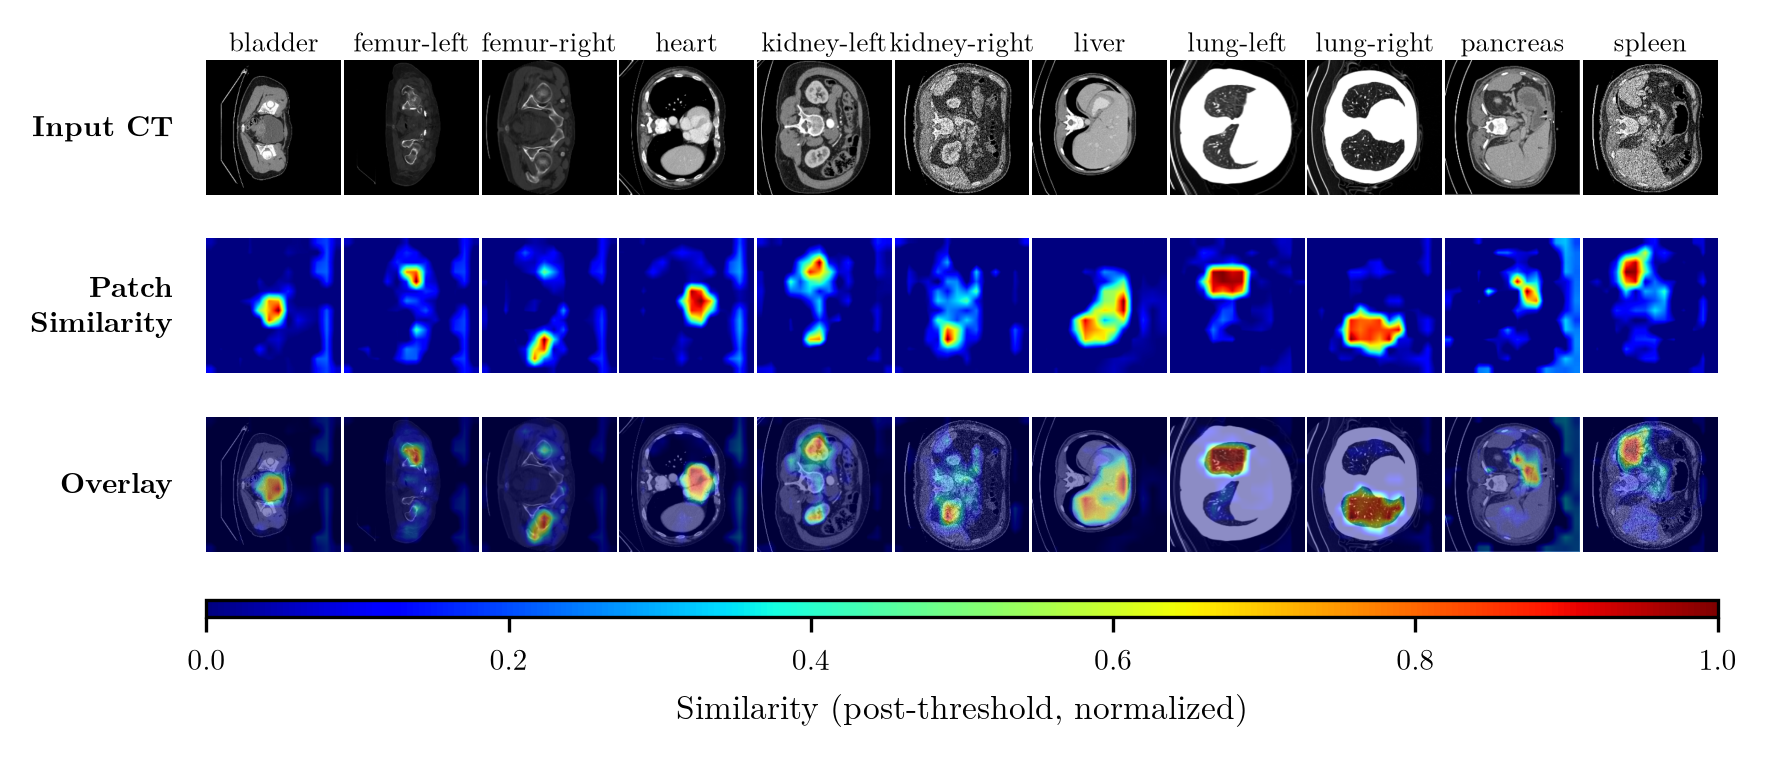
\includegraphics[width=\textwidth]{totalseg/totalseg_summary.png}
\caption{Generated masks on the TotalSegmentator test split, one column per
organ class. Large, high-contrast structures (lungs, liver, heart) are recovered
with clean boundaries from the prompt alone; the degradation on smaller,
lower-contrast structures (pancreas, kidneys) is visible as boundary spill
rather than as gross mislocalization, which is consistent with the per-class
ordering in Table~\ref{tab:perclass} and with the $14\times14$ patch grid
bounding attainable boundary precision.}
\label{fig:totalsegqual}
\end{figure}

\subsection{What the prompt actually contributes}
\label{sec:results:ablation}

A text-conditioned localizer invites an obvious objection: the text may be a
passenger, with the visual encoder doing all the work and the prompt serving
only as a class index. To test this we re-evaluated the fine-tuned v4 model with
five prompt formulations, changing only the text embedding and retraining
nothing (Table~\ref{tab:captions}).

\begin{table}[t]
\centering
\caption{Caption ablation. Text embeddings are the only variable; no retraining.
L5 is L4 with LEFT$\leftrightarrow$RIGHT and top$\leftrightarrow$bottom swapped.
We mark L4 because it is the formulation used during training, \emph{not}
because it wins. L2 and L4 are indistinguishable and in fact split the two
metrics: L2 is ahead on mIoU by 0.0006 (0.6273 vs.\ 0.6267) and L4 is ahead on
Dice by 0.0006 (0.7441 vs.\ 0.7435).}
\label{tab:captions}
\begin{tabular}{llrr}
\toprule
Level & Prompt formulation & mIoU & Dice \\
\midrule
L1 & Class name only                                  & 0.607 & 0.728 \\
L2 & Generic clinical caption                         & 0.627 & 0.743 \\
L3 & Position only (organ name removed)               & 0.561 & 0.684 \\
L4$^{*}$ & Full anatomical description (used in training) & 0.627 & 0.744 \\
L5 & Adversarial (L4 with position words swapped)     & 0.458 & 0.583 \\
\bottomrule
\end{tabular}
\end{table}

\begin{figure}[t]
\centering
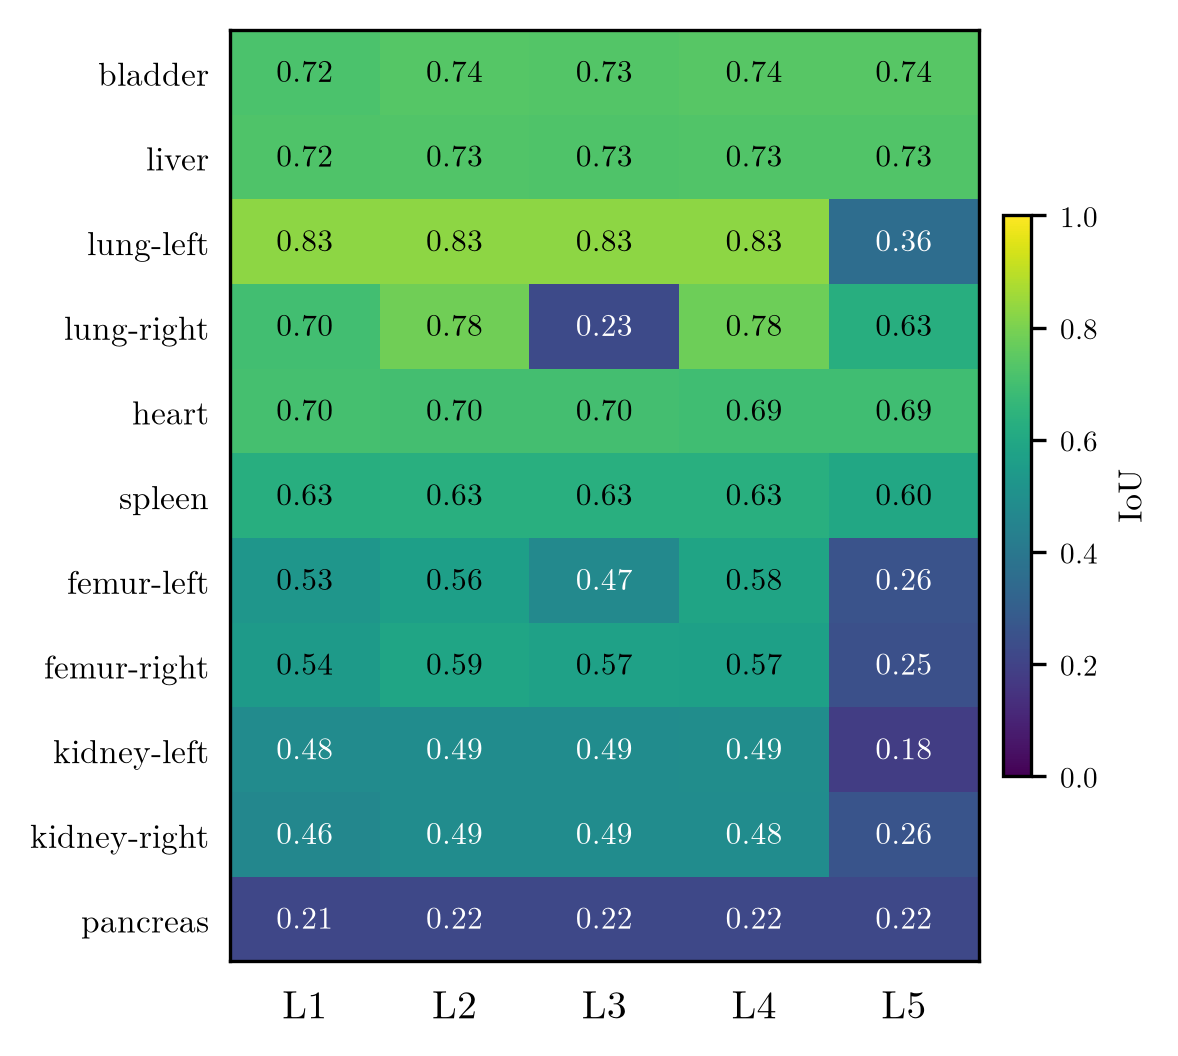
\includegraphics[width=0.74\textwidth]{caption_ablation.png}
\caption{Per-class IoU across the five prompt formulations, with bilateral pairs
placed adjacently and groups ordered easy to hard, so each pair can be read
against itself. Three features are visible directly. Classes whose identity
rests on a laterality word collapse in the L5 column (kidney-left
$0.49\to0.18$, femurs $\approx 0.58\to0.26$, lung-left $0.83\to0.36$) while
uniquely-positioned classes are untouched by the same transformation (liver,
heart, bladder all unchanged to two decimals). The exception is instructive:
\org{lung-right} falls only $0.78\to0.63$, because its prompt asserts a
three-lobe morphology that survives a laterality swap, which is the mechanism of
finding 3a. The isolated dark cell at \org{lung-right}/L3 is the accidental
two-word prompt error discussed in the text, not a property of the L3 level, as
\org{lung-left} holds 0.83 in the same column. Pancreas is flat across the
entire row including L1, the clearest single statement that it is data-limited
rather than prompt-limited.}
\label{fig:captionheat}
\end{figure}

Four findings follow, and Figure~\ref{fig:captionheat} shows the per-class
structure behind them.

\textbf{(1) Class names carry most of the signal, and elaboration adds almost
nothing.} L1 reaches 96.9\% of L4's mIoU. Fine-tuning made the
organ-name-to-region mapping strong enough that a single word recovers nearly
everything a multi-sentence anatomical description provides. Anatomical detail
does not buy the remaining 3\% either. A one-line generic clinical caption (L2)
matches the full description (L4) to within 0.0006 on both metrics, and the two
split them: L2 is ahead on mIoU, L4 on Dice. We take that as a cleaner statement
of equivalence than either ordering alone would be. Whatever L1 is missing is
supplied by having \emph{any} sentence context at all, not by the anatomy
written into it.

\textbf{(2) Position language refines rather than substitutes.} L3, which keeps
position cues but removes organ identity, scores \emph{below} L1 (0.561 vs.\
0.607). The model needs to know what to look for before where becomes useful.

\textbf{(3) The text is not a passenger.} Under L5, classes that depend on
left/right disambiguation collapse (kidney-left $-63\%$, lung-left $-57\%$,
femurs $-56\%$) while organs with unique positions are unaffected (liver,
spleen, heart, bladder). The model demonstrably uses the positional content of
the prompt, and corrupting it degrades exactly the classes for which it matters.

\textbf{(3a) Adversarial robustness scales with position-invariant anatomical
content.} The two lungs receive the same L5 transformation and respond very
differently: lung-left falls $0.83\to0.36$ ($-57\%$), lung-right only
$0.78\to0.63$ ($-19\%$). The prompts explain the asymmetry. Lung-left's
distinguishing clause, \emph{``slightly smaller than the right due to the heart
pushing into the left hemithorax''}, inverts cleanly under the swap and ends up
describing the other lung, leaving nothing pointing at the correct organ.
Lung-right's prompt contains a clause the swap cannot corrupt: \emph{``Three
lobes are present, divided by fissures visible as thin lines.''} The right lung
genuinely has three lobes and the left has two, so that sentence still points at
the right lung however the position words are flipped. We regard this as
actionable rather than incidental: including morphological cues that are
invariant under position swaps (lobe count, characteristic shape) hardens a
bilateral class against precisely the failure mode L5 probes.

\textbf{(4) Pancreas is data-limited, not prompt-limited.} Pancreas IoU stays at
0.21--0.22 across \emph{every} level, including L1 (the bare word ``pancreas'')
and L4. Prompt engineering will not fix pancreas. The ceiling is inherent to our
approach for small, low-contrast structures.

\paragraph{An unintended natural experiment.}
We auto-generated the L3 prompts, and the one for \org{lung-right} came out
wrong in both of its content words. It read \emph{``The left lung occupies the
left half of the image''} where our L4 convention requires \emph{``The right
lung \ldots{} the left half.''} The organ name is wrong \emph{and} the position
is wrong, and the two errors are mutually consistent: the resulting sentence is
a valid description of the \emph{left} lung. The model did not become confused
or degrade gracefully. It followed the prompt and segmented the left lung. IoU
on \org{lung-right} at L3 fell to 0.23, while \org{lung-left} at L3 held at
0.829, essentially identical to its 0.828 at L4, confirming the L3 \emph{level}
is not itself harmful for lungs and isolating the cause to the two wrong words.

A two-word error in one of eleven prompts therefore cost 55 IoU points on the
affected class. More importantly, it shows the failure is \emph{directional}
rather than degradative: a wrong-but-internally-coherent prompt yields a
confident segmentation of the wrong structure. For clinical deployment we regard
that as a considerably more dangerous failure mode than low confidence, because
nothing in the output signals that anything went wrong.

\subsection{Comparison to supervised and weakly-supervised references}
\label{sec:results:comparison}

\paragraph{Fully-supervised ceiling.}
Table~\ref{tab:fullysup} places our per-class Dice against TotalSegmentator
\cite{wasserthal2023totalsegmentator}, a fully-supervised 3D nnU-Net
\cite{isensee2021nnunet} trained on the same dataset with dense per-voxel
labels.

\begin{table}[t]
\centering
\caption{Against the fully-supervised reference. \textbf{The two columns are not
the same metric and must not be subtracted}; see the caveat below.
$\dagger$~TotalSegmentator v1 segments the heart as separate chambers; range
spans myocardium (0.937) to left ventricle (0.955). $\ddagger$~Lungs are
segmented per-lobe; left $=$ upper/lower (0.971/0.985), right $=$
upper/middle/lower (0.944/0.975/0.988).}
\label{tab:fullysup}
\begin{tabular}{lrr}
\toprule
Organ & OrganPrompt Dice (2D, weakly sup.) & TotalSegmentator Dice (3D, fully sup.) \\
\midrule
Liver        & 0.893 & 0.965 \\
Spleen       & 0.768 & 0.983 \\
Kidney left  & 0.627 & 0.953 \\
Kidney right & 0.595 & 0.939 \\
Pancreas     & 0.419 & 0.887 \\
Bladder      & 0.796 & 0.934 \\
Femur left   & 0.722 & 0.914 \\
Femur right  & 0.706 & 0.942 \\
Heart        & 0.866 & 0.937--0.955$^\dagger$ \\
Lung left    & 0.875 & 0.971/0.985$^\ddagger$ \\
Lung right   & 0.897 & 0.944--0.988$^\ddagger$ \\
\bottomrule
\end{tabular}
\end{table}

\textbf{Metric caveat.} We report 2D per-slice Dice on organ-present axial
slices; TotalSegmentator reports 3D volumetric Dice over whole volumes. 2D slice
Dice on organ-present slices is systematically \emph{more forgiving}, because no
empty or partial-boundary slices drag the average down. The true
supervised-to-weakly-supervised gap is therefore \emph{wider} than the raw
column difference suggests, and we recommend reading the second column as an
approximate upper bound achievable \emph{with} full pixel supervision, not a
like-for-like benchmark.

With that caveat applied, the pattern is still informative. On large,
high-contrast organs we reach 0.87--0.90 slice Dice with no pixel labels, and
the gap widens exactly where weak supervision is expected to struggle: pancreas
0.42 vs.\ 0.89, kidneys 0.60--0.63 vs.\ 0.94--0.95.

\paragraph{Weakly-supervised methods, stratified by supervision strength.}
``Weakly supervised'' spans a wide range of annotation cost, and that range
drives the comparison. Point- and scribble-supervised methods receive per-image
\emph{spatial} information that we never see: a scribble already answers
``where,'' which is the entire problem we solve from text alone. We include them
in Table~\ref{tab:weaksup} for context and note explicitly that they are not
like-for-like.

\begin{table}[t]
\centering
\small
\caption{Published weakly-supervised methods, ordered by supervision strength.
Entries reporting relative gains cannot be placed on the same axis as absolute
Dice, and no row here shares both a dataset and a metric with our work.}
\label{tab:weaksup}
\begin{tabularx}{\textwidth}{@{}l l X X@{}}
\toprule
Method & Supervision & Task / dataset & Reported Dice \\
\midrule
\textbf{OrganPrompt (this work)} & \textbf{Image-level text} & 11 organs, TotalSegmentator (2D) & \textbf{0.42--0.90} (mean 0.742) \\
MedCLIP-SAMv2, zero-shot \cite{koleilat2025medclipsamv2} & Text, no masks & BUSI, brain MRI, COVID-QU-Ex, lung CT & 78.21 mean DSC \\
MedCLIP-SAMv2, weakly sup.\ \cite{koleilat2025medclipsamv2} & Text $+$ pseudo-labels & same four tasks & 82.11 mean DSC \\
PET-CT lesion CAM \cite{fruh2021petct} & Image-level & Tumor lesions, PET-CT & 0.47 median (vs.\ 0.72 fully sup.) \\
Probabilistic-aware \cite{jiang2024probabilistic} & Point & BTCV (CT), CHAOS (MRI) & $+18.1\%/+10.2\%$ over prior point sup. \\
Probabilistic-aware \cite{jiang2024probabilistic} & Scribble & BTCV (CT), CHAOS (MRI) & $+58.4\%/+17.6\%$ over prior scribble sup. \\
\bottomrule
\end{tabularx}
\end{table}

Three caveats apply before comparing any two rows. The datasets differ, since
BTCV, AMOS and WORD are the usual multi-organ weak-supervision benchmarks rather
than TotalSegmentator. The metrics differ, both in the 2D/3D sense above and
because MedCLIP-SAMv2 reports DSC on a 0--100 scale over a different organ set
entirely. And two entries report relative gains, because that is what the source
publishes. We deliberately do not compute a ``gap'' between any two rows of this
table.

Within the image-level tier, which is the only strictly comparable one, our
per-organ range (0.42--0.90) sits above the image-level PET-CT CAM result (0.47
median), on a different task. Our closest methodological relative is
MedCLIP-SAMv2 \cite{koleilat2025medclipsamv2}, which shares the BiomedCLIP
backbone and the text-driven premise but pairs it with SAM
\cite{kirillov2023sam} for mask refinement instead of reading patch similarity
directly. We regard that difference as the point of comparison rather than the
scores: delegating mask formation to a second model makes the pipeline stronger,
and also makes it impossible to attribute a failure to the prompt, which is what
our caption ablation in \S\ref{sec:results:ablation} depends on being able to
do.

An earlier version of this comparison included a representative
scribble-supervised multi-organ CT result. We removed it. We could not trace the
figures to a specific publication, and an untraceable row is worse than an
absent one in a table whose whole purpose is to calibrate expectations. Our
honest summary of the point- and scribble-supervised tier is therefore
qualitative: those methods receive a per-image spatial hint that answers
``where,'' report 3D volumetric Dice on different organ sets, and we do not
measure ourselves against them here. What Table~\ref{tab:fullysup} already
establishes is the shape that matters: our deficit concentrates in small,
low-contrast structures (pancreas, kidneys) and nearly closes for large,
high-contrast ones.

\subsection{Bone-metastasis proximity index}
\label{sec:results:index}

The second half of our work applies the same frozen patch-similarity model to a
different question: given a vertebral metastasis, which organ is it closest to
invading? Figure~\ref{fig:organgrid} shows all 11 organ maps on a thoracic
lesion slice from Spine-Mets-CT-SEG \cite{pieper2024spinemets}, a dataset and CT
protocol our model was never trained on.

\begin{figure}[t]
\centering
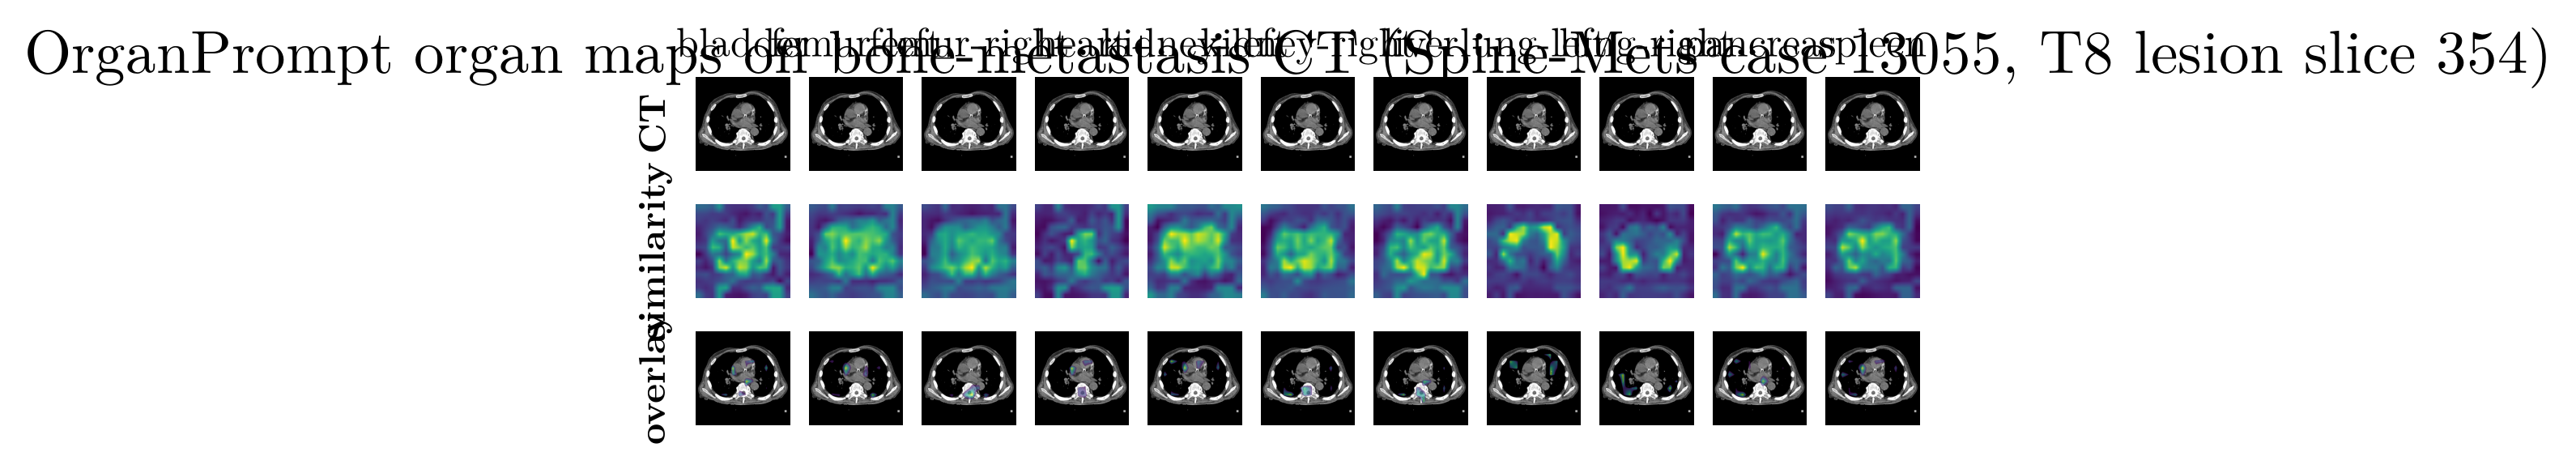
\includegraphics[width=\textwidth]{fig4_spine_organ_grid.png}
\caption{All 11 organ maps on a single Spine-Mets thoracic lesion slice (case
13055, T8 lesion). Rows: CT, raw patch-text similarity, overlay. We highlight
the top 2\% of each slice's own similarity distribution rather than an absolute
cutoff, because raw similarity is routinely negative across an entire slice and
organs win relatively rather than absolutely, so an absolute-zero threshold
renders most panels blank. We show the T8 \emph{lesion} slice rather than the
patient's peak-tumor slice, which sits at the pelvis where heart, lungs, liver
and spleen are out of frame; that slice would display noise in those columns and
wrongly imply the model hallucinates organs that are in fact absent.}
\label{fig:organgrid}
\end{figure}

Across the 46 labelled patients our index has mean 0.139 and median 0.083, with
9 patients below 0.01 and a smaller cluster of clearly-involved cases in the
0.25--0.50 range (maximum 0.500). Figure~\ref{fig:indexdist} shows the
distribution and Figure~\ref{fig:lesionoverlays} shows what low, mid and high
scores look like. We read the right-skewed shape as the expected mix of indolent
and locally aggressive metastases, not a calibration artifact.

\begin{figure}[t]
\centering
\begin{subfigure}{0.48\textwidth}
  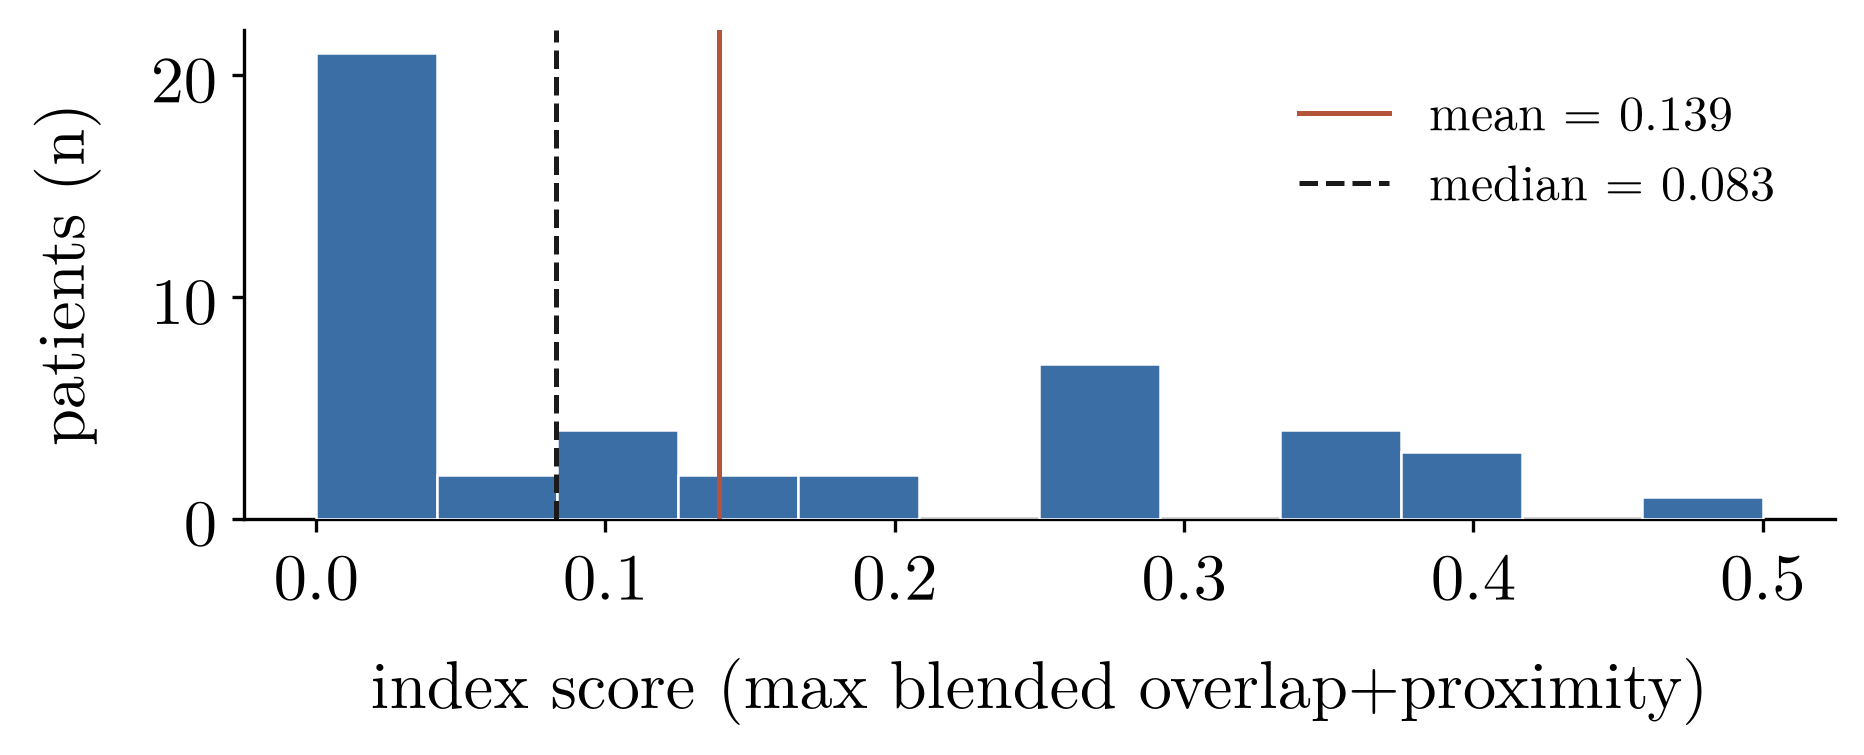
\includegraphics[width=\textwidth]{fig2_index_dist.png}
  \caption{}\label{fig:indexdist}
\end{subfigure}\hfill
\begin{subfigure}{0.48\textwidth}
  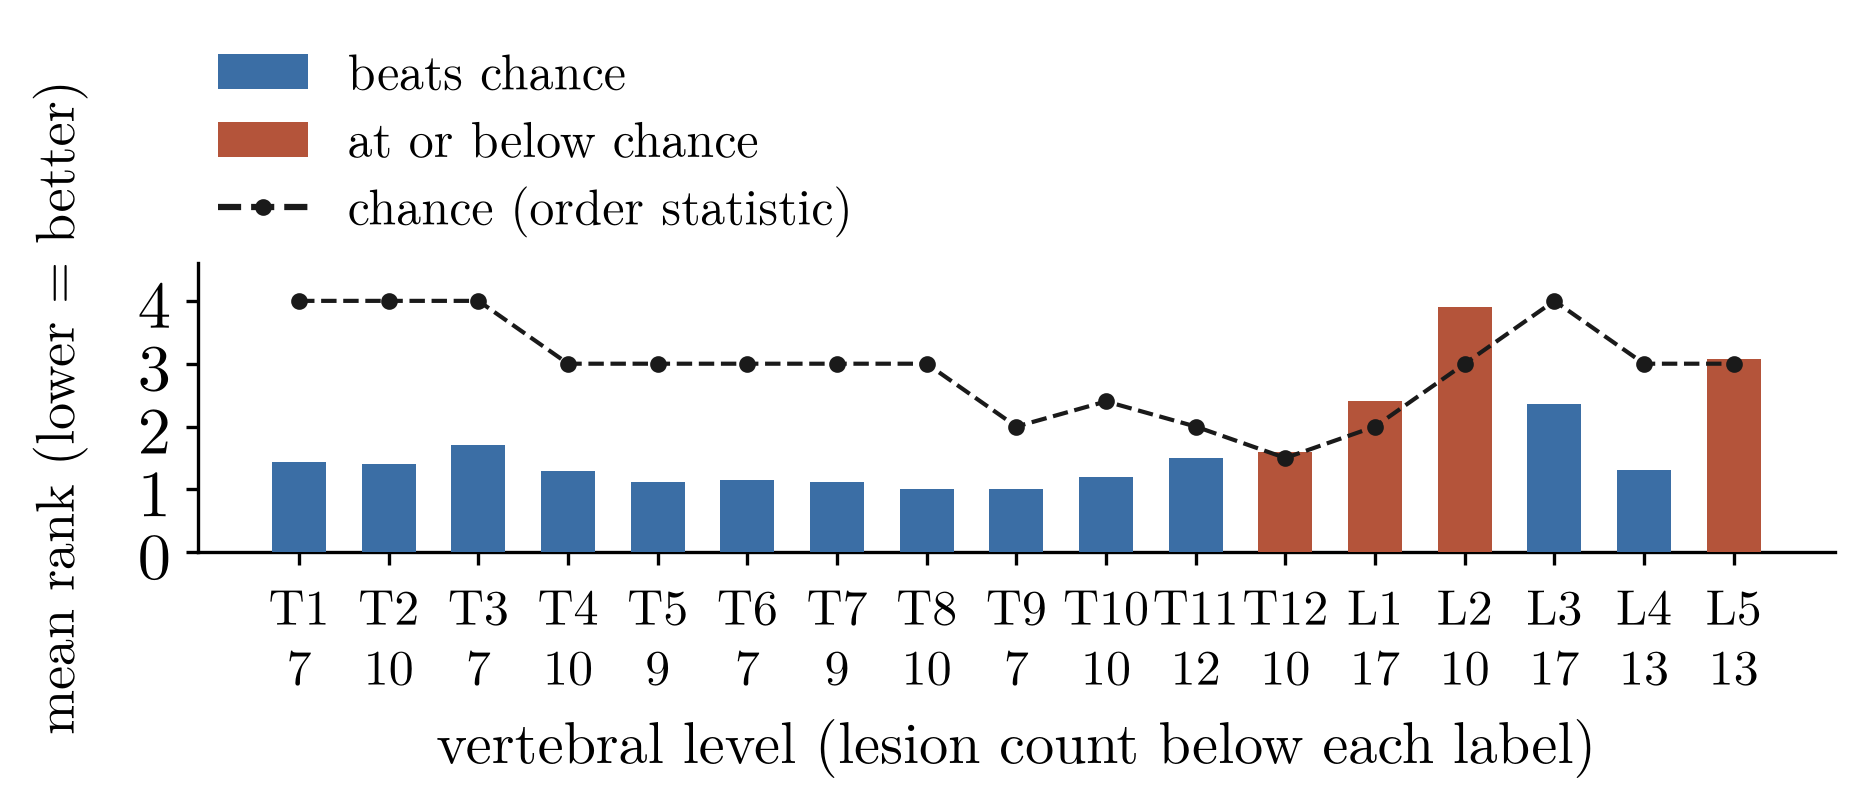
\includegraphics[width=\textwidth]{fig1_per_level.png}
  \caption{}\label{fig:perlevel}
\end{subfigure}
\caption{(\subref{fig:indexdist}) Per-patient index score across $n=46$
labelled patients, on the unleaked calibration. (\subref{fig:perlevel})
Per-vertebral-level mean rank of the correct organ(s) against that level's
chance mean rank (grey dashed). We derive bar colour from each level's own
observed-vs-chance comparison. $n$ per level is annotated inside each bar.}
\end{figure}

\begin{figure}[t]
\centering
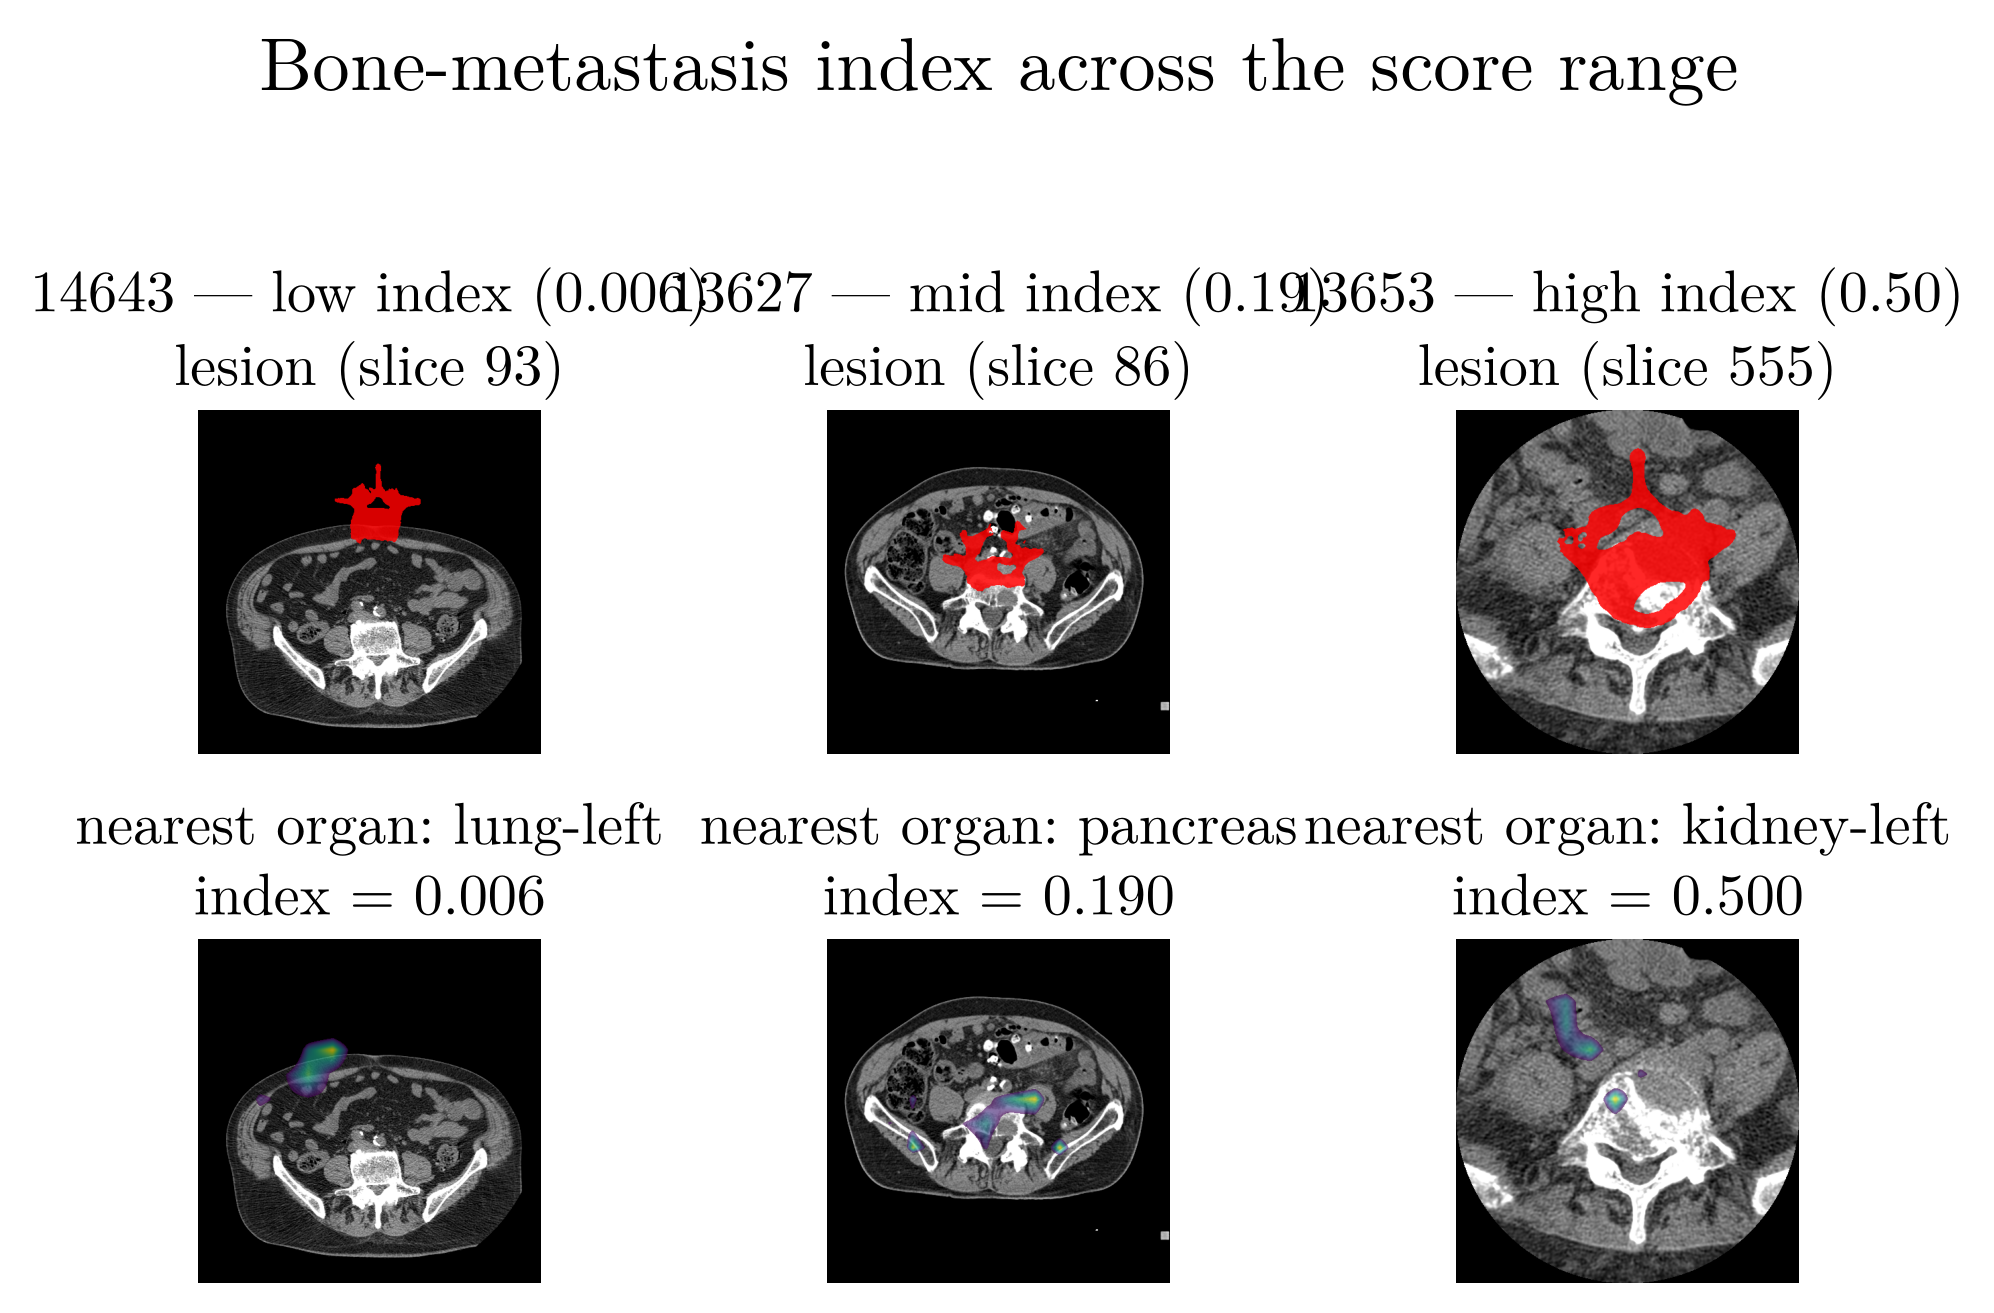
\includegraphics[width=\textwidth]{fig5_spine_lesion_overlays.png}
\caption{Three patients spanning the index range: 14643 (0.006), 13627 (0.190),
13653 (0.500, the cohort maximum). Top: ground-truth lesion mask on the
peak-tumor slice. Bottom: similarity map for the highest-scoring organ against
that lesion. The progression is the point: at low index the nearest-organ map
sits well away from the lesion, and at high index it is effectively touching it.
The low-index panel names \org{lung-left} as nearest organ at a pelvic slice.
This is a phantom detection of the kind we characterize in
\S\ref{sec:results:lesion}, and we retain rather than hide it because the low
index value correctly reflects that nothing real is near this lesion.}
\label{fig:lesionoverlays}
\end{figure}

\subsection{Per-lesion validation}
\label{sec:results:lesion}

Per-patient validation caps out at 20 evaluation points, namely patients with
exactly one involved vertebral level. Scoring per lesion instead, one point per
labelled vertebra and still one inference pass per patient, raises this to 180
lesions across 46 patients, of which 178 are rankable.

Our metric is the rank of the nearest anatomically expected organ in the model's
distance-ordered list, so chance depends on how many organs are expected at that
level and we compute it as the corresponding order statistic
$(n_{\text{organs}}+1)/(k+1)$ for $k$ expected organs.

\textbf{Mean rank is 1.78} (95\% CI $[1.56, 2.03]$), against a chance mean rank
of 2.91, with permutation $p < 0.0001$, and chance lies outside the confidence
interval. Top-1 accuracy is 0.622 and top-3 is 0.894. All our uncertainty
estimates resample \emph{patients}, never lesions: 180 lesions from 46 patients
are not 180 independent trials, since lesions within a patient share a scan and
a set of organ maps. Treating them as independent would inflate significance by
roughly the square root of the average lesions-per-patient, about $2\times$
here, which is larger than any effect our method changes produced.

\paragraph{The result is structured by level, not uniform.}
We consider Figure~\ref{fig:perlevel} the more informative view. Every thoracic
level T1--T11 beats chance, with T8 and T9 perfect (mean rank 1.00). L3 and L4
beat chance clearly. Four levels (T12, L1, L2 and L5) sit at or below chance.
The failure is therefore localized to the thoracolumbar junction rather than
distributed across the method.

\paragraph{A ground-truth error, found and corrected from the literature.}
Our expected-organ table originally dropped the lungs abruptly after T10.
Anatomical sources place the caudal extent of the costophrenic recess at T11 or
below, never above it, so the table was wrong and we corrected it on that basis.
We decided the correction from the literature \emph{before} applying it, and we
did not select it by checking which variant improved the metric. It moved mean
rank $1.94 \to 1.78$ and anatomically impossible top-1 detections $38 \to 34$.
Appendix~\ref{app:anatomy} reproduces the reasoning and sources.

It also moved T11 from below chance to above it, for two compounding reasons:
the answer key at that level became correct, and the expected set became larger,
which lowers chance there. Our earlier descriptions of this result named
``T11--L2'' as the failure band. The correct band after the fix is T12--L2 plus
L5. We now derive band membership in the figure from each level's own
observed-versus-chance comparison rather than from a hardcoded list of level
names, so this particular staleness cannot recur.

\paragraph{Residual failures.}
34 of 180 lesions top-rank an anatomically impossible organ, concentrated in
bladder and femur phantoms. Counting top-rank wins by class makes the
concentration explicit: \org{bladder} takes top rank on 29 lesions, 21 of them
anatomically wrong and 8 correct, while \org{femur-left} and \org{femur-right}
take top rank on 14 lesions of which \emph{none} are correct. The femur classes
never rank first at a level where a femur is expected.
Figure~\ref{fig:qualitative} contrasts a correct detection with one of these
phantoms and shows what the model is actually responding to.

\begin{figure}[t]
\centering
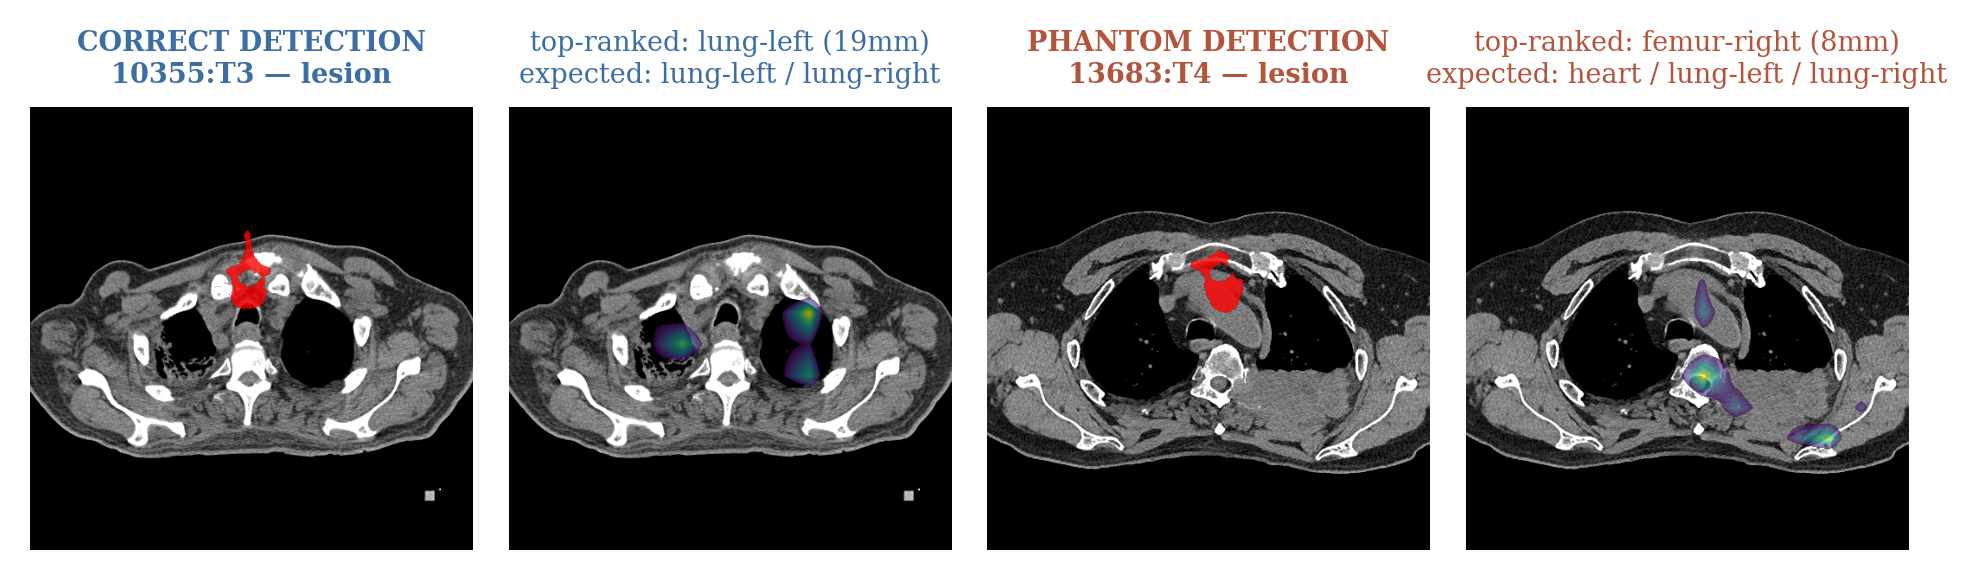
\includegraphics[width=0.58\textwidth]{fig3_qualitative.png}
\caption{Correct localization versus a phantom. Left: CT at the lesion's peak
axial position with the ground-truth mask (red). Right: raw patch-text
similarity for the top-ranked organ at that slice, thresholded to the top 2\% of
that slice's own distribution. \textbf{Top:} case 10355, T3, with
\org{lung-left} correctly ranked first at 19\,mm. \textbf{Bottom:} case 13683,
T4, with \org{femur-right} incorrectly ranked first at 8\,mm, ahead of heart,
\org{lung-left} and \org{lung-right}. The highlighted patches sit on rib
cross-sections at three separate points around the chest wall, not on any
structure resembling a femur shaft.}
\label{fig:qualitative}
\end{figure}

\subsection{Two negative results on the phantom failure mode}
\label{sec:results:negatives}

We tested two hypotheses for the phantom pattern. We fixed both configurations
in advance and report them as run, without retuning.

\paragraph{Field of view: rejected.}
The simplest explanation is that phantom patients' scans do not extend far
enough caudally to contain the true organ, so a wrong organ wins by default. Our
header-only scan-coverage measurement rejects this: phantom patients have
\emph{more} caudal coverage than clean ones (median 122\,mm vs.\ 88.5\,mm below
the last segmented vertebra), and 9 of 12 reach L5.

\paragraph{Missing vocabulary classes.}
Our text-encoder-only diagnostic showed that the \org{femur} prompt embeds
almost identically to an undefined \org{humerus} prompt, more closely than to
any of femur's own defined classmates, and that the \org{bladder} prompt's
nearest neighbour is an undefined \org{aorta} prompt. This motivated us to add
rib, humerus and aorta as negative prompts.

\paragraph{Calibration variants.}
Table~\ref{tab:variants} reports both variants. We adopt neither.

\begin{table}[t]
\centering
\small
\caption{Calibration variants, each a single pre-registered run.
\textbf{Both variants predate our T11/T12 ground-truth correction} and are
scored against the stricter pre-fix expected-organ table, so their comparator is
the pre-fix baseline row (mean rank 1.94), not the current headline 1.78. That
difference is the answer key changing, not the method. Chance moves with the key
too: 3.01 pre-fix, 2.91 post-fix.}
\label{tab:variants}
\begin{tabular}{@{}llrrrrrr@{}}
\toprule
Variant & Key & \makecell{Mean\\rank} & Top-1 & Top-3 & Ranked & \makecell{Imposs.\\top-1} & \makecell{Pair\\splits} \\
\midrule
\textbf{Baseline, current} & post-fix & \textbf{1.78} & 0.62 & 0.89 & 178/180 & 34/180 & 34/540 \\
Baseline, pre-fix \emph{(comparator)} & pre-fix & 1.94 & 0.59 & 0.86 & 178/180 & 38/180 & 34/540 \\
$+$ rib/humerus/aorta negatives & pre-fix & 2.04 & 0.53 & 0.82 & 171/180 & 37/180 & 58/540 \\
Z-score floor ($\mu + 2\sigma$) & pre-fix & 1.82 & 0.50 & 0.83 & 164/180 & 79/180 & 0/540 \\
\bottomrule
\end{tabular}
\end{table}

Global hard negatives traded one confusion for another. Femur pair-splitting
improved sharply ($31 \to 4$), but a \emph{new} lung pair-splitting problem
appeared ($0 \to 46$ of 540), and top-1 and top-3 both fell. The mechanism is
specific: we subtracted the rib negative from \emph{every} organ's score rather
than only from femur's, so it bled into the lungs' own scoring at the rib-lung
boundary, where lung tissue legitimately abuts rib.

The z-score floor moved mean rank in the right direction ($1.94 \to 1.82$) and
eliminated bilateral pair splitting entirely ($34 \to 0$ of 540), but more than
doubled anatomically impossible detections ($38 \to 79$). Nearly every wrong
detection wins at 0--1\,mm, which is consistent with the floor being too
permissive: instead of correctly vanishing where an organ is absent, most organs
retain a sliver of territory almost everywhere, and a sliver is enough to win a
proximity contest.

One methodological caution applies to reading Table~\ref{tab:variants}. Both
variants leave more lesions unrankable than the baseline (171 and 164 vs.\ 178),
so their mean ranks average over a smaller and easier subset, which flatters
that column. Top-1 and top-3 are computed over all 180 and are the cleaner
comparison. Both variants fall on those, which points the same way as the
impossible-detection counts.

\section{Discussion}
\label{sec:discussion}

\subsection{What text supervision buys, and where it stops}

We find that performance tracks organ size and contrast almost monotonically
(Table~\ref{tab:perclass}), which is the shape expected for a method with no
spatial supervision. The prompt must select a region by appearance and position
alone, and both cues degrade together for small, low-contrast structures.

The pancreas result is the sharpest statement of the ceiling, because
it is invariant to the one thing we can freely change. We measure pancreas IoU
at 0.213--0.218 across \emph{all five} of our prompt formulations: the bare word
``pancreas,'' a generic clinical caption, position-only text, the full
multi-sentence anatomical description, and the adversarial variant. A manipulation that moves the other classes by 60 percentage points moves the
pancreas by half a point. We conclude that whatever limits the pancreas here is
not in the text, so prompt engineering will not repair it. The constraint we run
into is that a small, low-contrast, elongated structure does not present a
$14\times14$-patch signature the encoder can separate from surrounding soft
tissue.

The distinction between prompt-limited and data-limited classes is worth drawing
explicitly, because the two call for different responses. The kidneys sit at 0.45--0.49 IoU and collapse by 47--63\% under adversarial
position swaps, which tells us they depend heavily on the positional text and
are therefore prompt-limited: better laterality cues should help them. The pancreas does not move under any prompt manipulation at all, so no amount of
prompt engineering will recover it, and the productive direction is a finer
patch grid or a different backbone. Reading only the aggregate mIoU would hide
that difference and invite us to spend effort in the wrong place.

\subsection{What the patch objective actually contributed}

The largest single gain comes from adding the patch-level loss, which moves mIoU
from 0.063 to 0.307. The size of that step is the most informative
number in Table~\ref{tab:progression}, because it quantifies how little
localization a globally-aligned model gives up for free. Before the patch loss
we were fine-tuning the same backbone with the same data and the same text
encoder, differing only in whether any objective required individual patch
tokens to be discriminative. Without such an objective, the patch tokens of a
contrastively trained encoder are optimized only insofar as they contribute to a
pooled embedding, and a pooled embedding can be correct while its constituents
are individually uninformative.

This is consistent with what the dense-alignment literature reports from the
opposite direction. MaskCLIP finds that CLIP retains more spatial information
than the pooled representation reveals, and recovers it by bypassing pooling
\cite{zhou2022maskclip}, and later work extends that recovery to weakly
supervised semantic segmentation \cite{yang2025clipdense}. Analyses of CLIP's
explainability reach a similar conclusion about why raw attention localizes
poorly \cite{li2024clipexplain}. We read our 0.063 measurement as the same
phenomenon observed without any recovery step: the information is latent rather
than absent, and something must either extract it or train it in.

We chose to train it in, and the reason generalizes. Extraction methods
recover \emph{where} an organ is, which is sufficient for segmentation
benchmarks. The downstream index additionally needs organ maps that vanish
where the organ is not present, because a proximity score computed against a
phantom mask is meaningless. That is a calibration property rather than a
localization one, and we found it easier to obtain from an objective that
explicitly pushes non-organ patches away than from a post-hoc reading of a model
never trained to express absence.

\subsection{Absence is information, and normalization destroys it}

The calibration correction added 0.059 mIoU and halved HD95 without retraining,
which makes it the cheapest improvement we report. The underlying lesson is more transferable than the number.

Per-image min--max normalization is close to a reflex when visualizing saliency,
and it is actively harmful here. Rescaling every slice to a fixed range forces a
slice containing no pancreas at all to span the same output range as a slice
centred on the pancreas. The relative ordering within each slice survives, but
the comparison \emph{between} slices, and therefore any notion of confidence,
does not. The raw similarities are bounded in $[-1,1]$ and routinely negative
across an entire slice, and that negativity is signal rather than noise: it is how the model expresses that the prompted organ is not here.

Any pipeline that reads similarity maps from a vision-language model should
check whether it is discarding this. The failure is silent, because
normalized maps look better in figures and score similarly on any metric
computed slice-by-slice among organ-present slices. It surfaces only when the
maps are asked a question that requires absolute comparison across slices, which
is exactly what the 3D index does.

\subsection{Elaboration is not what makes prompts work}

The caption ablation licenses a stronger conclusion than ``text matters.'' We
find the class name alone recovers 96.9\% of the full description's mIoU, and we
find the remaining gap is closed by a one-line generic clinical caption carrying
no anatomical content. L2 and L4 differ by 0.0006 on both metrics and split
them, with L2 ahead on mIoU and L4 ahead on Dice. The elaborate multi-sentence
descriptions we used throughout training therefore bought us nothing measurable
over a single generic sentence.

This matters practically, because writing those descriptions was the most
labour-intensive part of the setup, and the result says that labour was largely
wasted. Anyone extending this approach to a new organ set
should write class names and one-line captions, verify that this suffices, and
invest the saved effort in the failure modes below. One qualification applies: our descriptions were used during training as well as evaluation, so
we cannot separate the possibility that the model has already absorbed the
anatomical content from the possibility that the content was never necessary.
Distinguishing those would require retraining with short captions, which we did
not do.

The L3 result sharpens what the positional language is for. Position without
identity is actively worse than identity alone (0.561 vs.\ 0.607), so we
conclude the position clauses are not carrying the localization. They refine a
target the class name has already selected.

\subsection{Failure is directional, which is the safety-relevant finding}

The accidental error in the L3 \org{lung-right} prompt is the most operationally
important result in this paper, and we did not design it. The prompt named the wrong organ \emph{and} the wrong side, consistently, so it
became a valid description of the left lung. The model did not degrade, hedge,
or produce a diffuse map. It confidently segmented the left lung, and we measured
IoU on \org{lung-right} falling to 0.23 while \org{lung-left} at the same prompt
level held at 0.829, which proves the level itself was harmless and isolates the
cause to two words.

We therefore observe that a wrong-but-coherent prompt yields a confident
segmentation of the wrong structure. For any deployed system this is a worse
failure mode than low confidence, because nothing in the output signals
that anything went wrong. The mask is clean, well-formed, and anatomically
plausible. It is simply of a different organ. We argue that systems built on
text-prompted localization need prompt validation as a first-class component,
not an afterthought, because a wrong prompt does not announce itself downstream.

This failure mode is a direct consequence of the property the paper spends its
length establishing. A model that genuinely follows its prompt will follow a
wrong prompt just as faithfully as a right one, and the same evidence that
proves the text is load-bearing (finding 3) also proves that corrupting the text
is dangerous. This is not a defect specific to our pipeline. Any
method in which the prompt truly determines the output inherits it, and methods
that place a trained refiner between prompt and mask may partially mask the
symptom without removing the cause.

Finding 3a gives a concrete mitigation. We saw \org{lung-right} survive
the adversarial swap far better than \org{lung-left} ($-19.5\%$ vs.\ $-56.8\%$)
because its prompt contains a clause the swap cannot corrupt: the right lung
genuinely has three lobes and the left has two, so ``three lobes are present''
still points at the correct organ after every laterality word is flipped. We
conclude that prompt robustness is controllable by construction. If we include
morphological cues that are invariant under position swaps, such as lobe count,
characteristic shape, or vessel pattern, a bilateral class stops depending
entirely on laterality words it cannot verify. The swap test itself is cheap enough to be a routine design check: it
requires no retraining, and a class that collapses under it is a class whose
prompt rests entirely on assertions the image cannot confirm.

\subsection{Where our approach sits among dense-alignment methods}

We do not claim the best boundaries. DenseCLIP fine-tunes with a dense decoder
\cite{rao2022denseclip}, CLIPSeg attaches a transformer decoder emitting a
segmentation from a prompt \cite{lueddecke2022clipseg}, and MedCLIP-SAMv2 hands
mask formation to SAM \cite{koleilat2025medclipsamv2, kirillov2023sam}. All of
these will produce cleaner edges than an upsampled $14\times14$ grid.

What we gain by not doing this is attribution. Our caption ablation is
interpretable precisely because nothing sits between the prompt and the mask: a
55-point IoU drop can be traced to two words, because there is no intermediate
component that might have absorbed or amplified the error. Had a trained
decoder been in the path, we could not have said whether the decoder repaired a
bad localization or a good one was corrupted downstream. The architectural simplicity is the enabling
condition for the prompt findings rather than an oversight, and any attempt to
replicate those findings on a refiner-based pipeline would face this confound.

GLoRIA is the closest medical antecedent, learning global and local
representations jointly by matching sub-regions to report words
\cite{huang2021gloria}. The important difference is the supervision target. GLoRIA attends over words to build localized representations for
label-efficient recognition, whereas we supervise patch tokens directly against
a mask so the similarity map is the output rather than an intermediate. That
choice is what makes the map usable as geometry in our index, and it is also
what makes our failures legible as prompt failures.

\subsection{Our failure band is narrower than it first appears}

Describing T12--L2 and L5 as a uniform ``thoracolumbar failure'' overstates the
evidence, because those four levels fail in three different ways
(Table~\ref{tab:perlevel}).

\textbf{T12 and L5 are at chance, not below it.} We measure T12 missing by 0.10
rank (1.60 vs.\ 1.50) and L5 by 0.08 (3.08 vs.\ 3.00). T12 in particular faces the most stringent bar in the study: with seven expected organs its chance mean
rank is 1.50, so our model must rank a correct organ essentially first, every
time, to register any margin at all. Missing that bar by a tenth of a rank is not
comparable to failing a lenient one.

\textbf{L1 is a modest miss against a stringent bar}, at $+0.41$ against chance
2.00 with $k=5$.

\textbf{L2 is our only genuine failure}, at $+0.90$ against a lenient chance of
3.00 with only three expected organs. It is the one level where the model is
clearly worse than guessing, and it deserves to be reported as such
rather than averaged into a band.

\subsection{Two classes account for much of our damage}

The per-lesion detail identifies a more specific culprit than ``the lumbar spine
is hard.'' Across all 180 lesions we count the following.

\begin{itemize}
\item \org{bladder} takes top rank on 29 lesions, of which \textbf{21 are
      anatomically wrong and 8 correct}. It wins nearly three times more often
      where it does not belong than where it does.
\item \org{femur-left} and \org{femur-right} take top rank on 14 lesions, of
      which \textbf{zero are correct}. Our femur classes never once rank first
      at a level where a femur is anatomically expected, while winning 14 times
      where one is not.
\end{itemize}

This reframes our phantom problem. We are not looking at a generally-sound model
that occasionally misfires at difficult levels. Two of our eleven classes are
mislocalized in a way that produces false positives broadly and contributes
nothing where they would be correct. The two failing levels follow directly. At
L2, \org{bladder} hijacks top rank on 4 of 10 lesions at a level in the upper
lumbar spine where the bladder is nowhere near. At L5, the one level where
femurs \emph{are} expected, neither of our femur classes ever wins, and the
level's correct detections come from \org{bladder} instead.

It is unlikely to be coincidence that these are precisely the two classes the
text-only prompt diagnostic flagged. The \org{femur} prompt's appearance clause (``bright hyperdense cortical ring $\ldots$ central medullary canal'')
embeds almost identically to an undefined \org{humerus} prompt, more closely
than to any of femur's own defined classmates, and it describes a rib in
cross-section about as well as it describes a femur. The qualitative panel
(Figure~\ref{fig:qualitative}) confirms this visually: the winning
\org{femur-right} patches sit on rib cross-sections around the chest wall, on no
structure resembling a femoral shaft. The class is not localizing a femur at all. It is matching a generic cortical ring, and the 11-class vocabulary contains
nothing defined to outbid it.

These counts rest on small per-level samples ($n=10$ at L2, $n=13$ at L5) and
should be read as a diagnosis to act on rather than a precise effect size.

\subsection{Why both our calibration variants failed}

Both negative results have identified causes, which is what makes them worth
reporting rather than merely disclosing.

\textbf{Our global hard negatives failed by over-application, not by being the
wrong idea.} We added rib, humerus and aorta negatives to target exactly the
confusion we diagnosed above, and they worked on their intended target: femur
pair-splitting fell from 31 to 4. But we subtracted the negative from
\emph{every} organ's score rather than only from the classes it was meant to
correct, so it bled into the lungs' own scoring at the rib-lung boundary, where
lung tissue legitimately abuts rib, and created 46 new lung pair splits that had
not existed. The mechanism is specific and so is the fix it implies. We should
scope each negative to the classes we introduced it for, so that humerus and rib
compete only against our femurs and aorta only against our bladder. That per-organ-scoped variant has not
been run, and this result reads as ``wrong scoping'' rather than ``negatives do
not help.''

\textbf{Our z-score floor failed by permissiveness.} It eliminated bilateral
pair splitting entirely ($34 \to 0$) and improved mean rank against its correct
comparator ($1.94 \to 1.82$), but it more than doubled anatomically impossible
detections ($38 \to 79$). Both effects follow from one mechanism. A floor
set at $\mu + 2\sigma$ per organ is lenient enough that most organs retain a
sliver of territory almost everywhere instead of correctly vanishing where they
are absent. Slivers make bilateral territory symmetric, which zeroes our splits,
and a sliver is also enough to win a proximity contest at 0--1\,mm, which is
where nearly every new wrong detection landed.

\subsection{Evaluation-set discipline, and why we stop here}

The 180-lesion set has now absorbed several decisions: the calibration fit, the
bilateral-grouping change, the move from per-patient to per-lesion scoring, and
the two pre-registered calibration variants. It is a finite resource, and
continuing to test hypotheses against it would compound a multiple-comparisons
exposure that is already non-trivial.

This is our stated reason for not pursuing the residual phantom detections
further in this work, and we intend it to be read as a claim about what our
evaluation set can still support rather than a claim that nothing remains to be
found. The per-organ-scoped negative variant is the obvious next experiment, and the
right way to run it is against fresh data, or with
the exposure declared in advance, not as one more pass over the same 46
patients.

\subsection{Limitations of the localization method}

\textbf{Resolution.} Patch supervision is fixed at $14\times14$ by ViT-B/16 at $224\times224$.
Boundary precision is bounded by that grid, and the HD95 of 18.8\,px largely
reflects it. Raising input resolution is not a free fix: it changes the patch geometry our entire calibration and
mask-formation path is built around.

\textbf{Metric asymmetry.} All our Phase~1 numbers are 2D per-slice metrics on
organ-present slices, which is systematically more forgiving than 3D volumetric
scoring. Every cross-paper comparison here inherits that caveat, and the
supervised-to-weakly-supervised gap is wider than the tables' raw column
differences suggest.

\textbf{Prompt confound.} The anatomical descriptions were used during training
as well as at evaluation, so the caption ablation cannot fully separate ``the
description was never necessary'' from ``the model has already internalized the
description.'' Retraining with minimal captions would settle this, and we did
not do it.

\subsection{Limitations of the index}

\textbf{We use ground-truth tumor localization.} We attempt no weakly-supervised
tumor detection. We made this a scoping decision rather than an oversight:
adding a second layer of learned uncertainty before validating the index itself
would give us an uninterpretable result, since we could not attribute a failure
to the index or to the detector. It does mean our pipeline is not end-to-end
weakly supervised, and a deployed version would need that second stage.

\textbf{We fix our index parameters rather than fitting them.} We chose
$\alpha = \beta = 0.5$ and max-over-organs aggregation a priori. They are defensible but arbitrary, and no
sensitivity analysis over them is reported.

\textbf{Cohort.} We evaluate our index on 46 patients from a single collection,
with no external validation and no comparison against a clinical reference
standard for organ-involvement risk. Our per-level analysis rests on 7--17
lesions per level.

\textbf{Calibration provenance.} We originally fitted our per-organ constants on
the evaluation set, which made earlier versions of these numbers circular. We
now fit them on 35 held-out patients and every number here uses the corrected
constants, but the history is part of the record.

\textbf{Our expected-organ table may still be imperfect.} We found one error in
it and corrected it from anatomical literature, and that correction moved our
headline mean rank by 0.16 and shifted an entire level from below chance to
above it. The existence of one such error is evidence that others may remain, particularly in the same thoracolumbar region where the anatomy is
genuinely ambiguous. This is a real limit on how finely the per-level results
should be read.

\subsection{Future work}

The per-organ-scoped negative variant described above is the most specific next
step, because it addresses a mechanism we diagnosed rather than a
guess. Beyond that, we would harden our bilateral prompts with
position-invariant morphological cues, as our finding 3a implies, and adopt the
adversarial swap as a routine pre-deployment check. We would retrain with
minimal captions to resolve the prompt confound above. We would extend our index
to bone tumors as a distinct tissue target. And we would seek external
validation on an independent cohort, which the index most needs before any
clinical claim could be entertained.

\section{Conclusion}
\label{sec:conclusion}

Making patch-level text--image alignment an explicit training objective turns a
globally-aligned vision--language model into a text-prompted organ localizer,
recovering most of the localization signal for morphologically distinctive
structures without any per-pixel label at inference. The same frozen model
transfers to an unseen dataset and acquisition protocol to answer a downstream
clinical question, ranking the organ a vertebral metastasis is nearest to
invading well above chance across 180 lesions.

Two findings from that pipeline generalize past it. The first is that prompt
elaboration is not what makes text supervision work, because the class name
carries almost all of the signal and multi-sentence anatomical description adds
nothing measurable over a single generic sentence. The second is that when a
text-prompted localizer fails, it fails confidently, segmenting the wrong
structure cleanly rather than signaling uncertainty, which is why prompt
validation belongs in any deployed system as a first-class component.

Against those findings, our method remains bounded by the $14\times14$ patch
grid, by a two-class failure that we diagnose but do not repair, and by
single-cohort evaluation of the downstream index. The next experiment is
therefore specified by the diagnosis rather than chosen freely: we should scope
hard negatives to the classes they were introduced to correct, which is the one
change the failed global-negative result actually implicates.


\section*{Code and data availability}
Code, prompts, and all result JSON files are available at
\url{https://github.com/ArnavSangle/OrganPrompt}. The training and evaluation data is
TotalSegmentator v2.0.1 \cite{wasserthal2023totalsegdataset}; the bone-metastasis cohort
is Spine-Mets-CT-SEG \cite{pieper2024spinemets}, and the transfer sanity check uses
CT-ORG \cite{rister2020ctorg}. Model
checkpoints and the raw imaging data ($\sim$50\,GB) are not redistributed; every number
reported here is reproducible from the scripts named in the text.

\bibliographystyle{unsrtnat}
\bibliography{references}

\appendix
\section{Per-vertebral-level results}
\label{app:perlevel}

Table~\ref{tab:perlevel} gives the numeric values behind
Figure~\ref{fig:perlevel}. Chance is the order statistic for that level's
expected-organ set size, so it varies by level; a level ``beats chance'' when its
observed mean rank is strictly below its own chance value.

\begin{table}[H]
\centering
\caption{Per-vertebral-level mean rank against chance, post-correction. $n$ is
the number of rankable lesions at that level (178 of 180 total).}
\label{tab:perlevel}
\begin{tabular}{lrrrl}
\toprule
Level & $n$ & Mean rank & Chance & Verdict \\
\midrule
T1  &  7 & 1.43 & 4.00 & beats chance \\
T2  & 10 & 1.40 & 4.00 & beats chance \\
T3  &  7 & 1.71 & 4.00 & beats chance \\
T4  & 10 & 1.30 & 3.00 & beats chance \\
T5  &  9 & 1.11 & 3.00 & beats chance \\
T6  &  7 & 1.14 & 3.00 & beats chance \\
T7  &  9 & 1.11 & 3.00 & beats chance \\
T8  & 10 & 1.00 & 3.00 & beats chance (perfect) \\
T9  &  7 & 1.00 & 2.00 & beats chance (perfect) \\
T10 & 10 & 1.20 & 2.40 & beats chance \\
T11 & 12 & 1.50 & 2.00 & beats chance \\
T12 & 10 & 1.60 & 1.50 & at/below chance \\
L1  & 17 & 2.41 & 2.00 & at/below chance \\
L2  & 10 & 3.90 & 3.00 & at/below chance \\
L3  & 17 & 2.35 & 4.00 & beats chance \\
L4  & 13 & 1.31 & 3.00 & beats chance \\
L5  & 13 & 3.08 & 3.00 & at/below chance \\
\bottomrule
\end{tabular}
\end{table}

\section{All organ maps on a Spine-Mets slice}
\label{app:organgrid}

The index is computed from the 11 organ maps that Figure~\ref{fig:organgrid}
shows in full. It is reproduced here rather than in the body because eleven
columns cannot be read at single-column width, and because
\S\ref{sec:results:lesion} makes the argument it supports on the two cases in
Figure~\ref{fig:qualitative}, where the distinction between a correct detection
and a phantom is visible.

\begin{figure}[p]
\centering
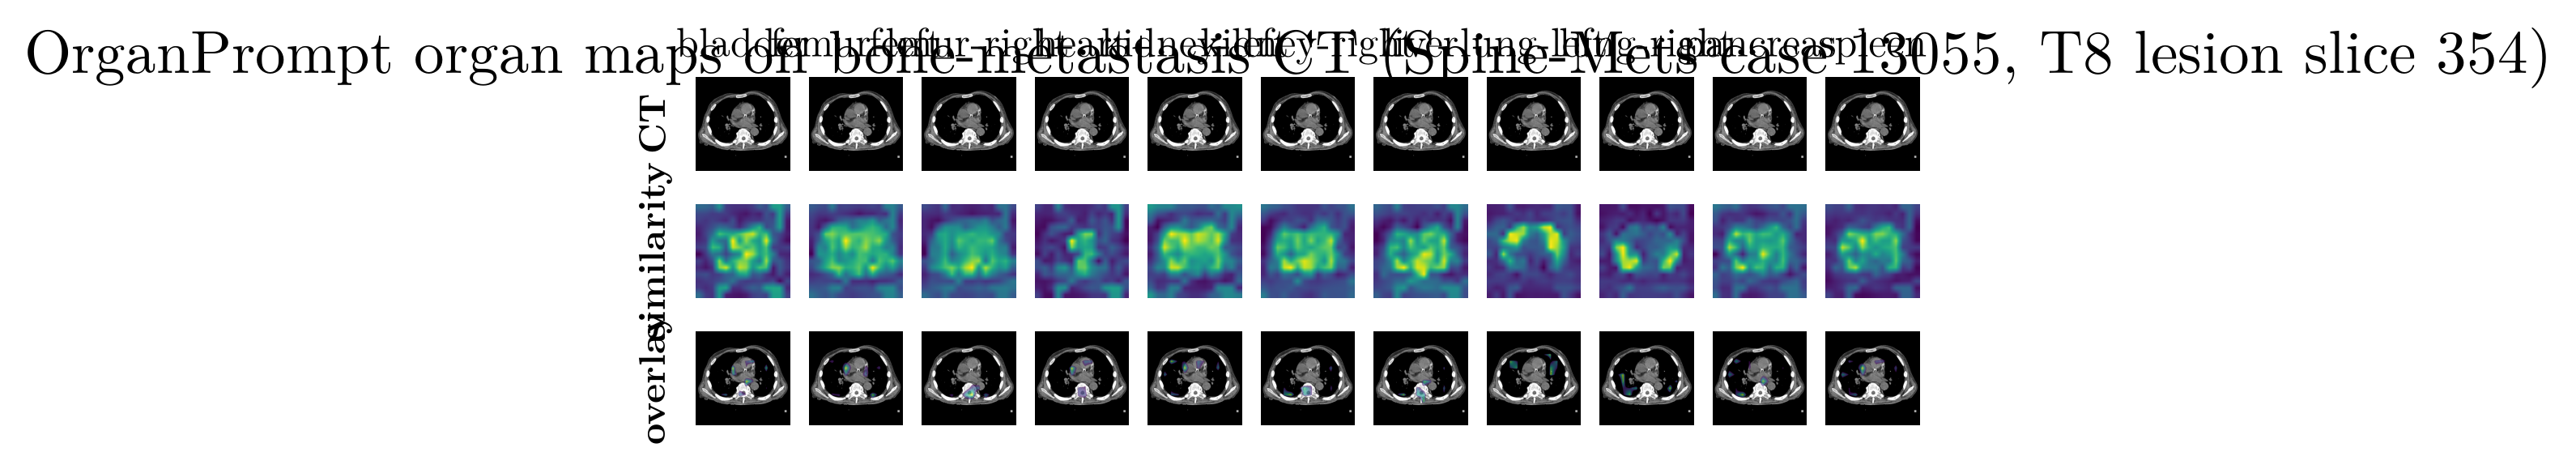
\includegraphics[width=\textwidth]{fig4_spine_organ_grid.png}
\caption{All 11 organ maps on a single Spine-Mets thoracic lesion slice (case
13055, T8 lesion). The rows are the CT slice, the raw patch-text similarity, and
the overlay. The highlight marks the top 2\% of each slice's own similarity
distribution rather than an absolute
cutoff, because raw similarity is routinely negative across an entire slice and
organs win relatively rather than absolutely, so an absolute-zero threshold
renders most panels blank. The panel is the T8 \emph{lesion} slice rather than
the patient's peak-tumor slice, which sits at the pelvis where heart, lungs,
liver and spleen are out of frame; that slice would display noise in those
columns and wrongly imply the model hallucinates organs that are in fact
absent.}
\label{fig:organgrid}
\end{figure}


% GENERATED by scripts/make_prompt_appendix.py -- do not edit by hand.
% Regenerate after any change to diagnostics/prompts_L*.json.

\section{Prompt formulations}
\label{app:prompts}

The caption ablation (\S\ref{sec:results:ablation}) varies only the text embedding. All five prompt sets are reproduced below verbatim, generated directly from the files the ablation consumed.

\subsection*{\texttt{bladder}}
\begin{description}[leftmargin=3.2em,style=nextline]
\item[\textbf{L1}] bladder
\item[\textbf{L2}] Axial CT scan of the bladder.
\item[\textbf{L3}] The urinary bladder is located in the top half of the image at the horizontal center, positioned symmetrically across the vertical midline.
\item[\textbf{L4}] Axial CT scan of the pelvis showing the urinary bladder as a smooth-walled fluid-filled hypodense oval. It sits at the horizontal center of the image in the top half, symmetric across the vertical midline. The rectum appears as a smaller structure at the bottom of the image behind it. The pubic symphysis is visible at the very top image edge in front of it. Wall thickness is thin and uniform.
\item[\textbf{L5}] Axial CT scan of the pelvis showing the urinary bladder as a smooth-walled fluid-filled hypodense oval. It sits at the horizontal center of the image in the bottom half, symmetric across the vertical midline. The rectum appears as a smaller structure at the top of the image behind it. The pubic symphysis is visible at the very bottom image edge in front of it. Wall thickness is thin and uniform.
\end{description}

\subsection*{\texttt{femur-left}}
\begin{description}[leftmargin=3.2em,style=nextline]
\item[\textbf{L1}] femur-left
\item[\textbf{L2}] Axial CT scan of the femur left.
\item[\textbf{L3}] The left femur is located on the right side of the image.
\item[\textbf{L4}] Axial CT scan of the thigh showing the left femur in transverse cross-section. Appears on the RIGHT side of the image as a bright hyperdense cortical ring surrounding lower-density cancellous bone with a central medullary canal. Adductor muscles border it toward the image center (medially). Vastus lateralis and iliotibial band flank it toward the right image edge (laterally).
\item[\textbf{L5}] Axial CT scan of the thigh showing the right femur in transverse cross-section. Appears on the LEFT side of the image as a bleft hyperdense cortical ring surrounding upper-density cancellous bone with a central medullary canal. Adductor muscles border it toward the image center (medially). Vastus lateralis and iliotibial band flank it toward the left image edge (laterally).
\end{description}

\subsection*{\texttt{femur-right}}
\begin{description}[leftmargin=3.2em,style=nextline]
\item[\textbf{L1}] femur-right
\item[\textbf{L2}] Axial CT scan of the femur right.
\item[\textbf{L3}] The right femur is located on the left side of the image.
\item[\textbf{L4}] Axial CT scan of the thigh showing the right femur in transverse cross-section. Appears on the LEFT side of the image as a hyperdense cortical ring with cancellous medullary interior. Adductor muscles border it toward the image center (medially). Vastus lateralis flanks it toward the left image edge (laterally). Slightly smaller cross-sectional area than the left femur in most individuals.
\item[\textbf{L5}] Axial CT scan of the thigh showing the left femur in transverse cross-section. Appears on the RIGHT side of the image as a hyperdense cortical ring with cancellous medullary interior. Adductor muscles border it toward the image center (medially). Vastus lateralis flanks it toward the right image edge (laterally). Slightly smaller cross-sectional area than the right femur in most individuals.
\end{description}

\subsection*{\texttt{heart}}
\begin{description}[leftmargin=3.2em,style=nextline]
\item[\textbf{L1}] heart
\item[\textbf{L2}] Axial CT scan of the heart.
\item[\textbf{L3}] The heart is located slightly right of center in the upper half of the image with its apex pointing toward the bottom-right.
\item[\textbf{L4}] Axial CT scan of the chest showing the heart within the pericardial sac. Appears slightly right of image center in the top half. The cardiac apex points toward the bottom-right of the image. The right ventricle is nearest the top of the image (most anterior), the left ventricle toward the bottom-right. Both lungs flank it — right lung on the image left, left lung on the image right. Pericardial fat appears as low-density material surrounding the cardiac silhouette.
\item[\textbf{L5}] Axial CT scan of the chest showing the heart within the pericardial sac. Appears slightly left of image center in the bottom half. The cardiac apex points toward the top-left of the image. The left ventricle is nearest the bottom of the image (most anterior), the right ventricle toward the top-left. Both lungs flank it — left lung on the image right, right lung on the image left. Pericardial fat appears as low-density material surrounding the cardiac silhouette.
\end{description}

\subsection*{\texttt{kidney-left}}
\begin{description}[leftmargin=3.2em,style=nextline]
\item[\textbf{L1}] kidney-left
\item[\textbf{L2}] Axial CT scan of the kidney left.
\item[\textbf{L3}] The left kidney is positioned on the right side of the image in the bottom half.
\item[\textbf{L4}] Axial CT scan of the upper abdomen showing the left kidney in the retroperitoneal space. Appears on the RIGHT side of the image in the bottom half. Its long axis runs roughly vertically. The renal hilum faces toward the image center (medially). The aorta is visible toward the bottom-center of the image just to its left. Perirenal fat surrounds the organ. Renal cortex is slightly brighter than the medullary pyramids.
\item[\textbf{L5}] Axial CT scan of the lower abdomen showing the right kidney in the retroperitoneal space. Appears on the LEFT side of the image in the top half. Its long axis runs roughly vertically. The renal hilum faces toward the image center (medially). The aorta is visible toward the top-center of the image just to its right. Perirenal fat surrounds the organ. Renal cortex is slightly blefter than the medullary pyramids.
\end{description}

\subsection*{\texttt{kidney-right}}
\begin{description}[leftmargin=3.2em,style=nextline]
\item[\textbf{L1}] kidney-right
\item[\textbf{L2}] Axial CT scan of the kidney right.
\item[\textbf{L3}] The right kidney is located on the left side of the image in the bottom half.
\item[\textbf{L4}] Axial CT scan of the upper abdomen showing the right kidney in the retroperitoneal space. Appears on the LEFT side of the image in the bottom half, slightly more toward the top than the left kidney. The renal hilum faces toward the image center (medially). The inferior vena cava is visible just to its right in the image. The liver occupies the top-left of the image directly above it.
\item[\textbf{L5}] Axial CT scan of the lower abdomen showing the left kidney in the retroperitoneal space. Appears on the RIGHT side of the image in the top half, slightly more toward the bottom than the right kidney. The renal hilum faces toward the image center (medially). The inferior vena cava is visible just to its left in the image. The liver occupies the bottom-right of the image directly above it.
\end{description}

\subsection*{\texttt{liver}}
\begin{description}[leftmargin=3.2em,style=nextline]
\item[\textbf{L1}] liver
\item[\textbf{L2}] Axial CT scan of the liver.
\item[\textbf{L3}] The liver occupies the left portion of the image extending toward the center in the top half.
\item[\textbf{L4}] Axial CT scan of the upper abdomen showing the liver. Dominates the LEFT portion of the image from the left edge toward and past the center, in the top half. The right lobe is largest and sits furthest left in the image. The left lobe tapers toward image center. Intrahepatic vessels (portal and hepatic veins) branch throughout as tubular structures. The gallbladder may appear as a small oval hypodense structure at the bottom of the liver mass.
\item[\textbf{L5}] Axial CT scan of the lower abdomen showing the liver. Dominates the RIGHT portion of the image from the right edge toward and past the center, in the bottom half. The left lobe is largest and sits furthest right in the image. The right lobe tapers toward image center. Intrahepatic vessels (portal and hepatic veins) branch throughout as tubular structures. The gallbladder may appear as a small oval hypodense structure at the top of the liver mass.
\end{description}

\subsection*{\texttt{lung-left}}
\begin{description}[leftmargin=3.2em,style=nextline]
\item[\textbf{L1}] lung-left
\item[\textbf{L2}] Axial CT scan of the lung left.
\item[\textbf{L3}] The left lung is located in the right half of the axial CT image.
\item[\textbf{L4}] Axial CT scan of the chest showing the left lung. Occupies the RIGHT half of the image as low-attenuation aerated tissue. The mediastinum and heart border it along the left side of the right half. The chest wall curves along the right image edge. Branching bronchial and vascular markings extend from the hilum toward the periphery. The left lung is slightly smaller than the right due to the heart pushing into the left hemithorax.
\item[\textbf{L5}] Axial CT scan of the chest showing the right lung. Occupies the LEFT half of the image as low-attenuation aerated tissue. The mediastinum and heart border it along the right side of the left half. The chest wall curves along the left image edge. Branching bronchial and vascular markings extend from the hilum toward the periphery. The right lung is slightly smaller than the left due to the heart pushing into the right hemithorax.
\end{description}

\subsection*{\texttt{lung-right}}
\begin{description}[leftmargin=3.2em,style=nextline]
\item[\textbf{L1}] lung-right
\item[\textbf{L2}] Axial CT scan of the lung right.
\item[\textbf{L3}] The left lung occupies the left half of the image. \textbf{[This prompt is erroneous; see Section 4.2. Reproduced as run.]}
\item[\textbf{L4}] Axial CT scan of the chest showing the right lung. Occupies the LEFT half of the image as low-attenuation aerated tissue. The mediastinum borders it along the right side of the left half. The chest wall curves along the left image edge. Three lobes are present, divided by fissures visible as thin lines. Branching bronchial and vascular markings radiate from the hilum. The right lung is larger than the left.
\item[\textbf{L5}] Axial CT scan of the chest showing the left lung. Occupies the RIGHT half of the image as low-attenuation aerated tissue. The mediastinum borders it along the left side of the right half. The chest wall curves along the right image edge. Three lobes are present, divided by fissures visible as thin lines. Branching bronchial and vascular markings radiate from the hilum. The left lung is larger than the right.
\end{description}

\subsection*{\texttt{pancreas}}
\begin{description}[leftmargin=3.2em,style=nextline]
\item[\textbf{L1}] pancreas
\item[\textbf{L2}] Axial CT scan of the pancreas.
\item[\textbf{L3}] The pancreas lies horizontally across the bottom half of the image, with its head on the left side, body crossing the center, and tail extending toward the right side.
\item[\textbf{L4}] Axial CT scan of the upper abdomen showing the pancreas in the retroperitoneal space. Lies horizontally across the bottom half of the image. The head (widest portion) is on the LEFT side of the image, nestled in the duodenal loop. The body crosses the center of the image. The tail extends toward the RIGHT side of the image, pointing toward the spleen. The superior mesenteric vessels appear as round structures just in front of the pancreatic body.
\item[\textbf{L5}] Axial CT scan of the lower abdomen showing the pancreas in the retroperitoneal space. Lies horizontally across the top half of the image. The head (widest portion) is on the RIGHT side of the image, nestled in the duodenal loop. The body crosses the center of the image. The tail extends toward the LEFT side of the image, pointing toward the spleen. The superior mesenteric vessels appear as round structures just in front of the pancreatic body.
\end{description}

\subsection*{\texttt{spleen}}
\begin{description}[leftmargin=3.2em,style=nextline]
\item[\textbf{L1}] spleen
\item[\textbf{L2}] Axial CT scan of the spleen.
\item[\textbf{L3}] The spleen is located on the right side of the image in the bottom half.
\item[\textbf{L4}] Axial CT scan of the upper left abdomen showing the spleen. Appears on the RIGHT side of the image in the bottom half. Its convex surface faces the right image edge and the lateral chest wall. Its concave hilum faces toward the image center-left. The stomach may be visible just to its left in the image. The left kidney is visible just below and behind it. Homogeneous soft tissue attenuation with a smooth capsule.
\item[\textbf{L5}] Axial CT scan of the lower right abdomen showing the spleen. Appears on the LEFT side of the image in the top half. Its convex surface faces the left image edge and the lateral chest wall. Its concave hilum faces toward the image center-right. The stomach may be visible just to its right in the image. The right kidney is visible just below and behind it. Homogeneous soft tissue attenuation with a smooth capsule.
\end{description}

\section{Anatomical basis for the expected-organ table}
\label{app:anatomy}

The correction described in \S\ref{sec:results:lesion} changes a headline
number, so the reasoning behind it is reproduced here rather than only cited. The
full source list, with quoted passages and the questions put to each source, is
in \code{docs/references/anatomy-citations.md} in the repository.

\paragraph{The question, asked before the change was made.}
Should the \code{EXPECTED} entries for T11 and T12 include the lungs? Put
anatomically: at typical inspiration, does the posterior lung base, via the
costophrenic recess, reach the T11 vertebral level, and the T12 level? Does this
differ by side, sex, or respiratory phase? The research was completed and the
answer fixed before the expected-organ table was edited and before the
validation was re-scored. This ordering matters, because the alternative
procedure, changing the table and keeping whichever version improves the metric,
would make the evaluation circular.

\paragraph{Primary quantitative source.}
Oh et al.\ \cite{oh2009retrodiaphragmatic} retrospectively reviewed 540
consecutive posteroanterior chest radiographs from general health screening, of
which 282 met inclusion criteria (clear visualization of the inferior boundary
of the posterior costophrenic sulcus behind the right hemidiaphragm, no
diaphragm-affecting abnormality; 155 men, 127 women, mean age
$40.7 \pm 8.4$ years). They measured the depth of the posterior costophrenic
sulcus below the diaphragmatic dome and scored its level against the spine.

The mean right posterior costophrenic sulcus depth was $29.2 \pm 15.6$\,mm, at
an average spinal level of $13.5 \pm 0.6$, which is the lower half of the L1
vertebral body: a full vertebral level below T12. Depth increased with height,
BMI and total diaphragmatic height, indicating normal population variation
rather than a rare tail. The authors' own conclusion is that a standard
posteroanterior chest radiograph must extend more than 3\,cm below the lateral
costophrenic sulcus, or to the L1 spine level, to capture the retrodiaphragmatic
lung fully.

Both T11 and T12 therefore sit at or above the population-average posterior
lung and pleural extent. A lung detected at either level is consistent with
normal anatomy and is not evidence of a phantom detection.

\paragraph{Triangulating sources.}
Three further references were consulted and agree on direction. A textbook-derived
thorax chapter states that lung tissue does not normally extend much below T10 in
quiet respiration, while the pleural cavity's inferior extent reaches
approximately T12 through the costodiaphragmatic recess, or lower along the
twelfth rib in the midscapular line, and flags these levels as approximate. A
descriptive anatomy reference for the costodiaphragmatic recess notes that during
deep inspiration the lungs descend up to two intercostal spaces into the recess.
A clinical teaching reference places the lower border of the lung at the
vertebral column at the upper half of T11 in moderate respiration, before any
inspiratory excursion is added.

The distinction that resolves the apparent disagreement between the T10 and
T11--L1 figures is that lung parenchyma in quiet breathing and the aerated lung
at inspiration are not the same boundary. The expected-organ table scores whether
a predicted lung mask could plausibly extend to a level, which tracks the
inspiratory and recess extent, not the resting position.

\paragraph{Points of convergence.}
Every source giving a specific level places the posterior lung base at T11 or
below: T11 in moderate respiration, approximately T12 for the recess, and the
lower half of L1 as a quantitative radiographic average. No source reported a
systematic left--right asymmetry large enough to justify treating the two lungs
differently. The Oh et al.\ study measured the right side specifically because
the right costophrenic sulcus is the one clearly visible below the liver and
diaphragm on a frontal film, which is a measurement-visibility constraint and
not a claim about the left side.

\paragraph{Decision, and what it changed.}
Both T11 and T12 include \org{lung-left} and \org{lung-right}. The weakest
single-source claim already places T11 within range, and T12 sits comfortably
below every conservative estimate. No source was found that would support
treating a lung detection at either level as anatomically impossible.

Applying the correction moved mean rank from 1.94 to 1.78, reduced anatomically
impossible top-1 detections from 38 to 34, and moved chance from 3.01 to 2.91,
since chance depends on expected-set size. It also moved T11 from below chance to
above it. As noted in \S\ref{sec:discussion}, the fact that one such error existed
is itself evidence that the table may contain others, particularly in this same
thoracolumbar region where the anatomy is genuinely variable.


\end{document}
